% =============================================================================
%  Diplomado en Data Science Aplicada con Python para la Toma de Decisiones
%  Clase 25: De clasificador a detector --- TL completo + intro a YOLO
%  Arca Continental Ecuador | UDLA
%  Compilar: pdflatex -shell-escape presentacion.tex (x2 para refs)
% =============================================================================
\documentclass[aspectratio=169, 11pt]{beamer}

\usepackage[T1]{fontenc}
\usepackage[utf8]{inputenc}
\usepackage[spanish,es-noshorthands]{babel}
\usepackage{FiraSans}
\usepackage{FiraMono}
\renewcommand{\familydefault}{\sfdefault}
\usepackage{graphicx}
\usepackage{tikz}
\usetikzlibrary{arrows.meta, positioning, shapes.geometric, shapes.misc,
  calc, fit, decorations.pathreplacing, backgrounds}
\usepackage{fontawesome5}
\usepackage{minted}
\usepackage{tcolorbox}
\tcbuselibrary{minted, skins, breakable}
\usepackage{booktabs}
\usepackage{colortbl}
\usepackage{multicol}
\usepackage{hyperref}
\usepackage{calc}
\usepackage{amsmath}

\definecolor{arcaRed}{HTML}{C82B40}
\definecolor{arcaDark}{HTML}{6B1525}
\definecolor{udlaCrimson}{HTML}{A31545}
\definecolor{arcaGray}{HTML}{F5F5F5}
\definecolor{arcaLightGray}{HTML}{EBEBEB}
\definecolor{textDark}{HTML}{2D2D2D}
\definecolor{textMuted}{HTML}{6B7280}
\definecolor{codeGreen}{HTML}{16A34A}
\definecolor{codeBlue}{HTML}{2563EB}
\definecolor{codeOrange}{HTML}{EA580C}
\definecolor{codePurple}{HTML}{7C3AED}

\usetheme{default}
\usecolortheme{default}
\setbeamertemplate{navigation symbols}{}
\setbeamertemplate{footline}{}
\setbeamertemplate{headline}{}
\setbeamercolor{normal text}{fg=textDark}
\setbeamercolor{frametitle}{fg=arcaRed, bg=white}
\setbeamercolor{title}{fg=white}
\setbeamercolor{subtitle}{fg=white!85}
\setbeamercolor{author}{fg=white!80}
\setbeamercolor{date}{fg=white!70}
\setbeamercolor{item}{fg=arcaRed}
\setbeamercolor{subitem}{fg=arcaDark}
\setbeamercolor{block title}{fg=white, bg=arcaRed}
\setbeamercolor{block body}{fg=textDark, bg=arcaGray}
\setbeamercolor{section in toc}{fg=arcaDark}
\setbeamerfont{frametitle}{size=\Large, series=\bfseries}
\setbeamerfont{title}{size=\huge, series=\bfseries}
\setbeamerfont{subtitle}{size=\large}
\setbeamerfont{author}{size=\normalsize}
\setbeamerfont{date}{size=\small}
\setbeamerfont{block title}{size=\normalsize, series=\bfseries}
\setbeamerfont{footnote}{size=\tiny}
\setbeamertemplate{itemize item}{\scriptsize\raise1.5pt\hbox{\color{arcaRed}$\blacktriangleright$}}
\setbeamertemplate{itemize subitem}{\scriptsize\raise1pt\hbox{\color{arcaDark}$\bullet$}}
\setbeamertemplate{enumerate items}[default]
\setbeamercolor{enumerate item}{fg=arcaRed}

\setbeamertemplate{headline}{%
  \begin{tikzpicture}[remember picture, overlay]
    \fill[arcaDark] (current page.north west) rectangle
      ([yshift=-0.7cm]current page.north east);
    \node[anchor=west, inner sep=0pt] at
      ([xshift=0.6cm, yshift=-0.35cm]current page.north west)
      {
\includegraphics[height=0.45cm]{../logo_udla_white.png}};
    \node[anchor=east, inner sep=0pt] at
      ([xshift=-0.6cm, yshift=-0.35cm]current page.north east)
      {
\includegraphics[height=0.45cm]{../ArcaContinental_white.png}};
  \end{tikzpicture}%
  \vspace{0.7cm}%
}

\setbeamertemplate{footline}{%
  \begin{tikzpicture}[remember picture, overlay]
    \node[anchor=south east, font=\scriptsize\bfseries\color{arcaRed}] at
      ([xshift=-0.5cm, yshift=0.15cm]current page.south east)
      {\insertframenumber};
  \end{tikzpicture}%
  \vspace{0.3cm}%
}

\setbeamertemplate{frametitle}{%
  \vspace{0.25cm}%
  \usebeamerfont{frametitle}\usebeamercolor[fg]{frametitle}\insertframetitle%
  \par\vspace{2pt}%
  \begin{tikzpicture}
    \fill[arcaRed] (0,0) rectangle (3cm, 1.5pt);
    \fill[arcaLightGray] (3cm,0) rectangle (\textwidth, 0.5pt);
  \end{tikzpicture}%
  \vspace{0.1cm}%
}

\newtcblisting{pyblock}[1][]{%
  listing engine=minted, minted language=python, minted style=friendly,
  minted options={fontsize=\small, linenos=false, breaklines=true, python3=true},
  colback=arcaGray, colframe=arcaRed, left=4pt, right=4pt, top=4pt, bottom=4pt,
  boxrule=0pt, leftrule=3pt, arc=2pt, listing only, #1}

\newcommand{\sectionframe}[2]{%
  \begingroup
  \setbeamertemplate{headline}{}%
  \setbeamertemplate{footline}{}%
  \begin{frame}[plain, noframenumbering]
    \begin{tikzpicture}[remember picture, overlay]
      \fill[arcaRed] (current page.south west) rectangle (current page.north east);
      \node[anchor=center, text=white, font=\Huge\bfseries, text width=12cm,
            align=center] at ([yshift=0.5cm]current page.center) {#1};
      \node[anchor=center, text=white!80, font=\large, text width=10cm,
            align=center] at ([yshift=-0.8cm]current page.center) {#2};
    \end{tikzpicture}
  \end{frame}
  \endgroup
}

\title{Diplomado en Data Science Aplicada\\con Python para la Toma de Decisiones}
\subtitle{Clase 25: De clasificador a detector}
\author{Carlos Enrique Mosquera Trujillo}
\date{8 de Mayo, 2026}

\begin{document}

% ── PORTADA ──────────────────────────────────────────────────────────────────
{
\setbeamertemplate{headline}{}
\setbeamertemplate{footline}{}
\begin{frame}[plain, noframenumbering]
  \begin{tikzpicture}[remember picture, overlay]
    \fill[arcaDark] (current page.south west) rectangle (current page.north east);
    \fill[arcaRed] ([yshift=-3.5cm]current page.north west) rectangle
      ([yshift=-4.2cm]current page.north east);
    \node[anchor=west, inner sep=0pt] at
      ([xshift=1cm, yshift=-1.5cm]current page.north west)
      {
\includegraphics[height=1cm]{../logo_udla_white.png}};
    \node[anchor=east, inner sep=0pt] at
      ([xshift=-1cm, yshift=-1.5cm]current page.north east)
      {
\includegraphics[height=1cm]{../ArcaContinental_white.png}};
  \end{tikzpicture}
  \vspace{2.5cm}
  \begin{center}
    {\usebeamerfont{title}\usebeamercolor[fg]{title}\inserttitle\par}
    \vspace{0.4cm}
    {\usebeamerfont{subtitle}\usebeamercolor[fg]{subtitle}\insertsubtitle\par}
    \vspace{0.6cm}
    {\usebeamerfont{author}\usebeamercolor[fg]{author}\insertauthor\par}
    \vspace{0.15cm}
    {\usebeamerfont{date}\usebeamercolor[fg]{date}\insertdate\par}
  \end{center}
\end{frame}
}

\begin{frame}[shrink]{Hoja de Ruta de Hoy}
  \vspace{4pt}
  \begin{center}
  \begin{tikzpicture}[
    node distance=0.25cm,
    roadstep/.style={rectangle, rounded corners=4pt, draw=arcaRed, fill=arcaRed!8,
                 minimum width=11.5cm, minimum height=0.55cm,
                 font=\footnotesize\bfseries\color{arcaDark}, align=left,
                 text width=10.5cm, inner sep=4pt},
    num/.style={circle, fill=arcaRed, text=white, font=\scriptsize\bfseries,
                minimum size=0.45cm, inner sep=0pt},
  ]
    \node[roadstep] (s0) {\hspace{0.7cm}Recap clase 25 + 5 tareas de visi\'on};
    \node[roadstep, below=of s0] (s1) {\hspace{0.7cm}Bounding boxes, IoU y \textbf{multi-output}};
    \node[roadstep, below=of s1] (s2) {\hspace{0.7cm}Sliding window: el detector ingenuo};
    \node[roadstep, below=of s2] (s3) {\hspace{0.7cm}YOLO + m\'etricas (mAP, precision, recall)};
    \node[roadstep, below=of s3] (s4) {\hspace{0.7cm}\textbf{Fine-tuning desde la necesidad}};
    \node[roadstep, below=of s4] (s5) {\hspace{0.7cm}\textbf{Somos un equipo de annotation} (Label Studio)};
    \node[roadstep, below=of s5] (s6) {\hspace{0.7cm}\textbf{Fine-tune en vivo} + OCR cascade};
    \node[roadstep, below=of s6] (s7) {\hspace{0.7cm}\textbf{App Gradio} con link p\'ublico};

    \foreach \i in {0,...,7}{
      \node[num] at ([xshift=0.4cm]s\i.west) {\the\numexpr\i+1};
    }
  \end{tikzpicture}
  \end{center}
\end{frame}

\begin{frame}[shrink]{D\'onde Quedamos en Clase 25}
  \vspace{6pt}
  {\footnotesize\color{arcaDark}\bfseries
    En la clase pasada construimos la base. Hoy aterrizamos el proyecto
    completo: equipo de etiquetado, fine-tune en vivo, app desplegada.}

  \vspace{14pt}
  {\footnotesize
  \begin{itemize}\setlength{\itemsep}{6pt}
    \item[{\color{arcaRed}\scriptsize\faCheck}]
      \textbf{Transfer learning} con VGG16 + Coca/Pepsi (proyecto colectivo).
    \item[{\color{arcaRed}\scriptsize\faCheck}]
      Limitaciones del MLP + por qu\'e CNN.
    \item[{\color{arcaRed}\scriptsize\faCheck}]
      C\'omo construir un buen dataset (5 reglas de oro).
    \item[{\color{codeGreen}\scriptsize\faArrowRight}]
      \textbf{Hoy:} extendemos a detecci\'on + OCR, etiquetamos en equipo,
      entrenamos en vivo, desplegamos como app.
  \end{itemize}
  }
\end{frame}

\sectionframe{Tareas de Visi\'on por Computadora}{Cinco maneras distintas de ``ver''}

\begin{frame}[shrink]{Las 5 Tareas Principales}
  \vspace{8pt}
  {\footnotesize
  \begin{tabular}{@{}p{3.0cm} p{4.5cm} p{5.0cm}@{}}
    \toprule
    \textbf{Tarea} & \textbf{Salida} & \textbf{Pregunta que responde} \\
    \midrule
    \rowcolor{arcaGray}
    \textbf{Clasificaci\'on}
    & 1 etiqueta por imagen
    & ?`Qu\'e hay en la imagen? \\
    \textbf{Detecci\'on}
    & N bounding boxes + clase
    & ?`Qu\'e hay y \emph{d\'onde}? \\
    \rowcolor{arcaGray}
    \textbf{Segmentaci\'on}
    & M\'ascara por pixel
    & ?`Qu\'e \emph{pixeles} son cada cosa? \\
    \textbf{Pose / keypoints}
    & Puntos clave conectados
    & ?`D\'onde est\'an las articulaciones? \\
    \rowcolor{arcaGray}
    \textbf{OCR}
    & Texto extra\'ido
    & ?`Qu\'e \emph{dice} la imagen? \\
    \bottomrule
  \end{tabular}
  }

  \vspace{14pt}
  \begin{tcolorbox}[colback=codeGreen!8, colframe=codeGreen, boxrule=0.5pt,
    arc=2pt, left=6pt, right=6pt, top=4pt, bottom=4pt]
    {\scriptsize\color{arcaDark}
    \faKey\hspace{4pt}\textbf{Hoy:} miramos cada una con un ejemplo,
    luego nos enfocamos en \textbf{detecci\'on}.}
  \end{tcolorbox}
\end{frame}

\begin{frame}[shrink]{1. Clasificaci\'on}
  \vspace{4pt}
  \begin{center}
    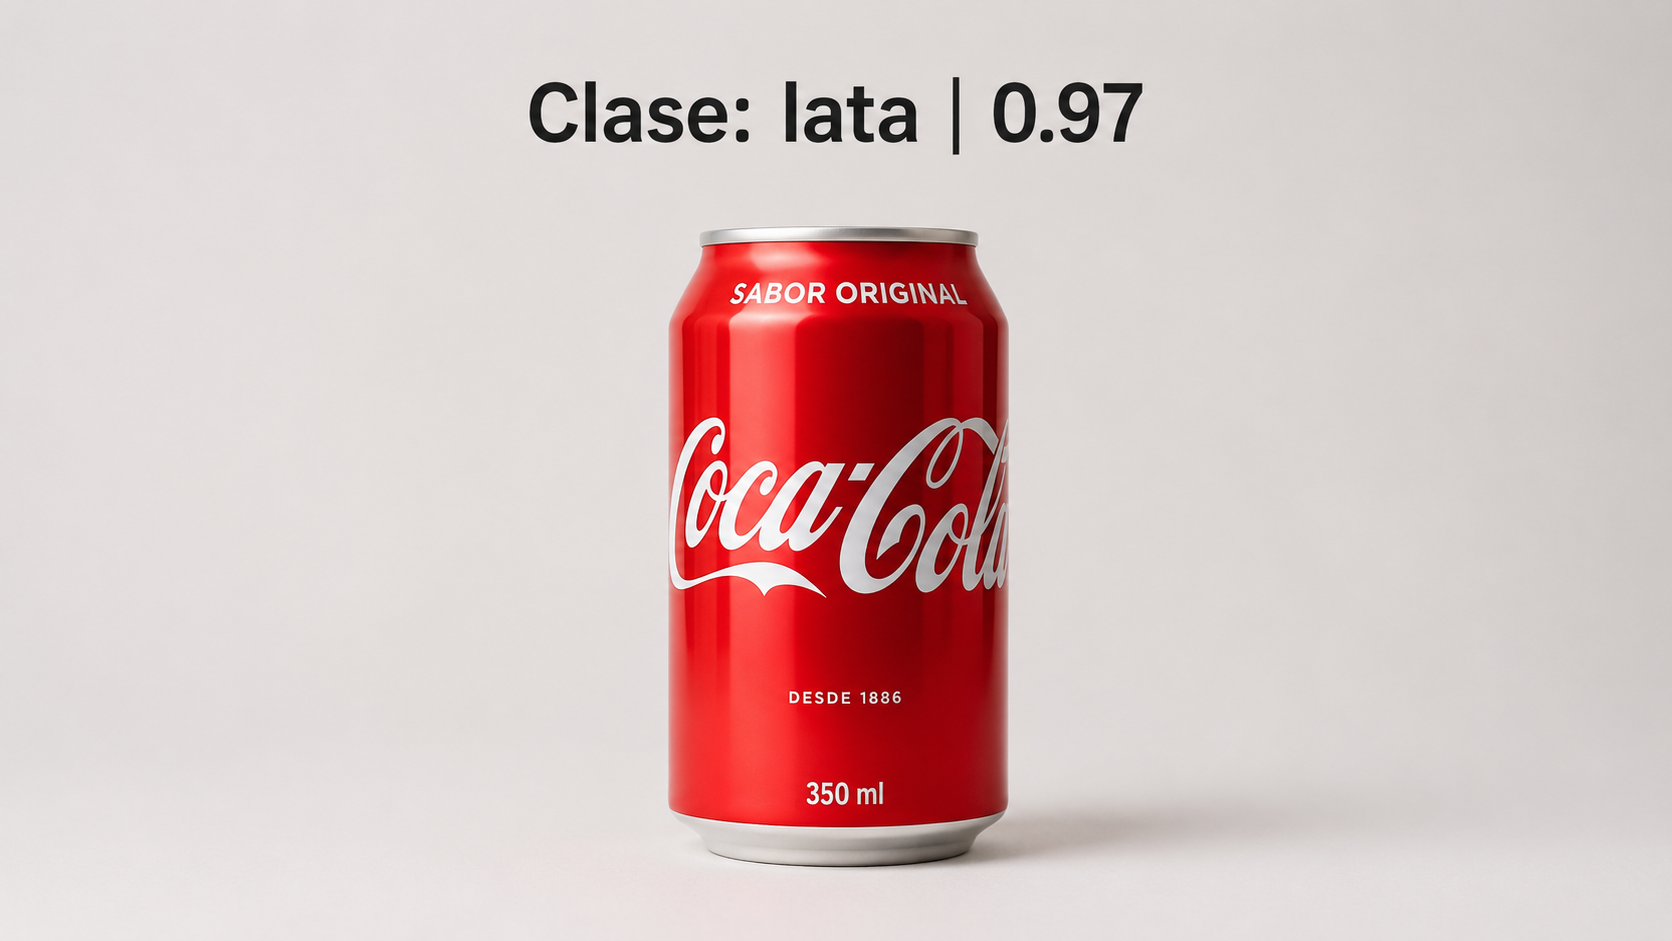
\includegraphics[width=0.55\textwidth]{fig_task_classification.png}
  \end{center}

  \vspace{4pt}
  {\footnotesize
  \begin{itemize}\setlength{\itemsep}{2pt}
    \item[{\color{arcaRed}\scriptsize\faArrowRight}]
      \textbf{Salida:} una etiqueta y su confianza (``lata'' 0.97).
    \item[{\color{arcaRed}\scriptsize\faArrowRight}]
      Asume que hay \textbf{un objeto principal} en la imagen.
    \item[{\color{arcaRed}\scriptsize\faArrowRight}]
      Lo que hicimos en clases 22--24: MNIST, Fashion MNIST, Cats vs Dogs, Coca vs Pepsi.
  \end{itemize}
  }
\end{frame}

\begin{frame}[shrink]{2. Detecci\'on}
  \vspace{4pt}
  \begin{center}
    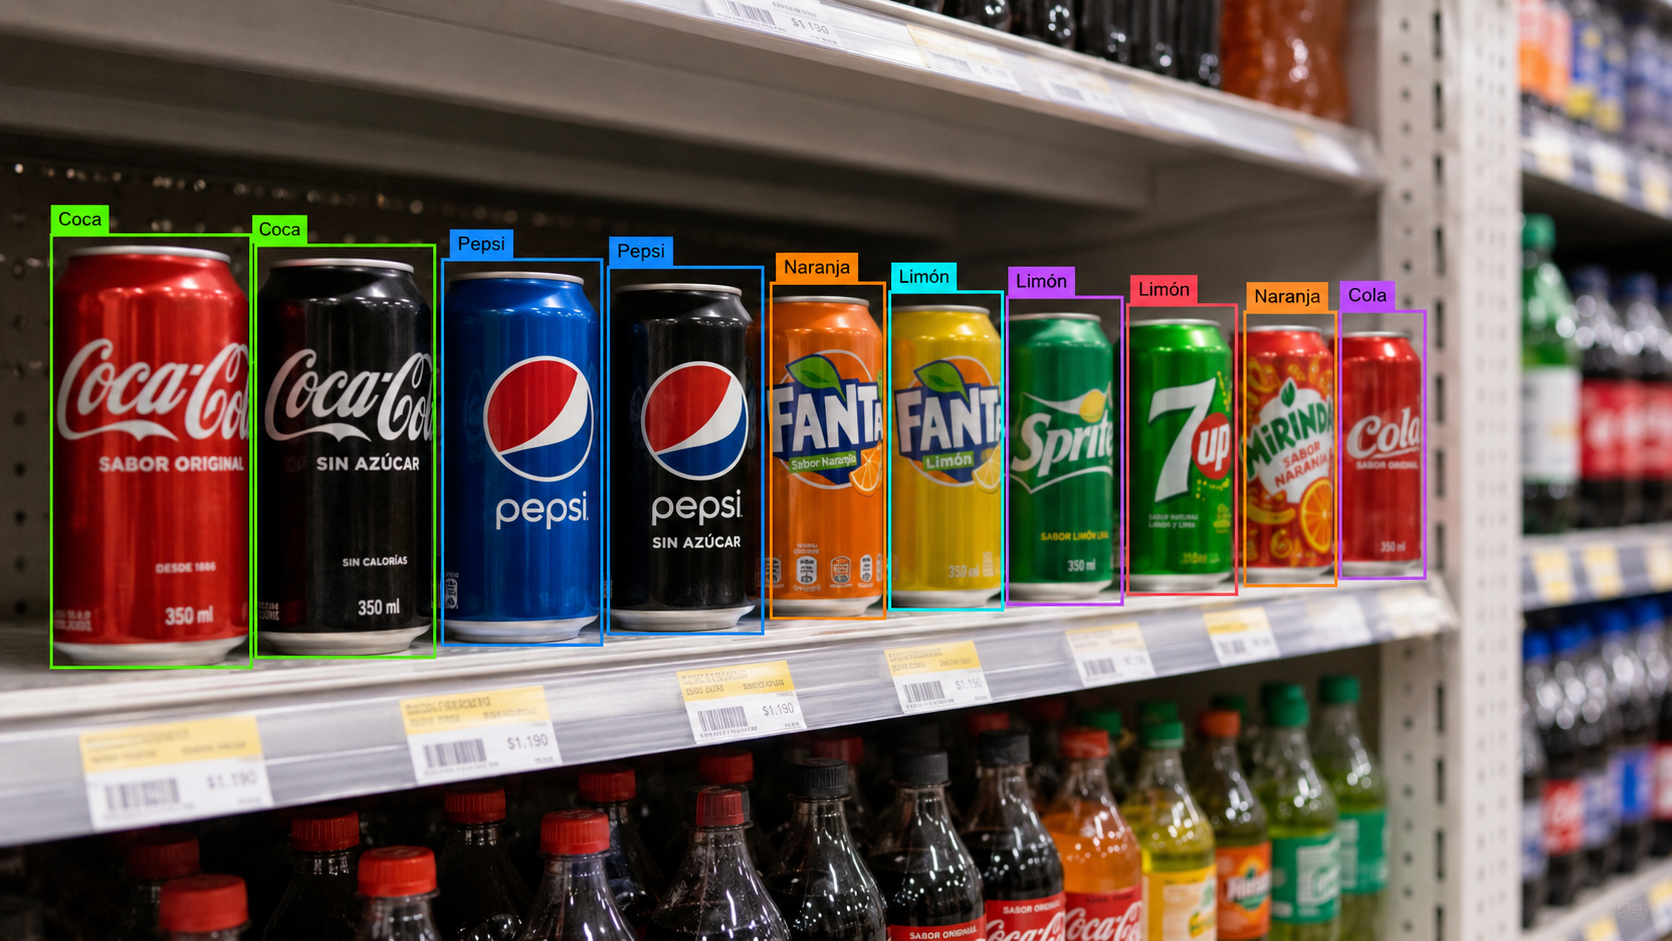
\includegraphics[width=0.78\textwidth]{fig_task_detection.png}
  \end{center}

  \vspace{4pt}
  {\footnotesize
  \begin{itemize}\setlength{\itemsep}{2pt}
    \item[{\color{arcaRed}\scriptsize\faArrowRight}]
      \textbf{Salida:} lista de bboxes \texttt{(x, y, w, h, clase)}, una por objeto.
    \item[{\color{arcaRed}\scriptsize\faArrowRight}]
      Maneja \textbf{m\'ultiples objetos} simult\'aneos en una sola imagen.
  \end{itemize}
  }
\end{frame}

\begin{frame}[shrink]{3. Segmentaci\'on}
  \vspace{4pt}
  \begin{center}
    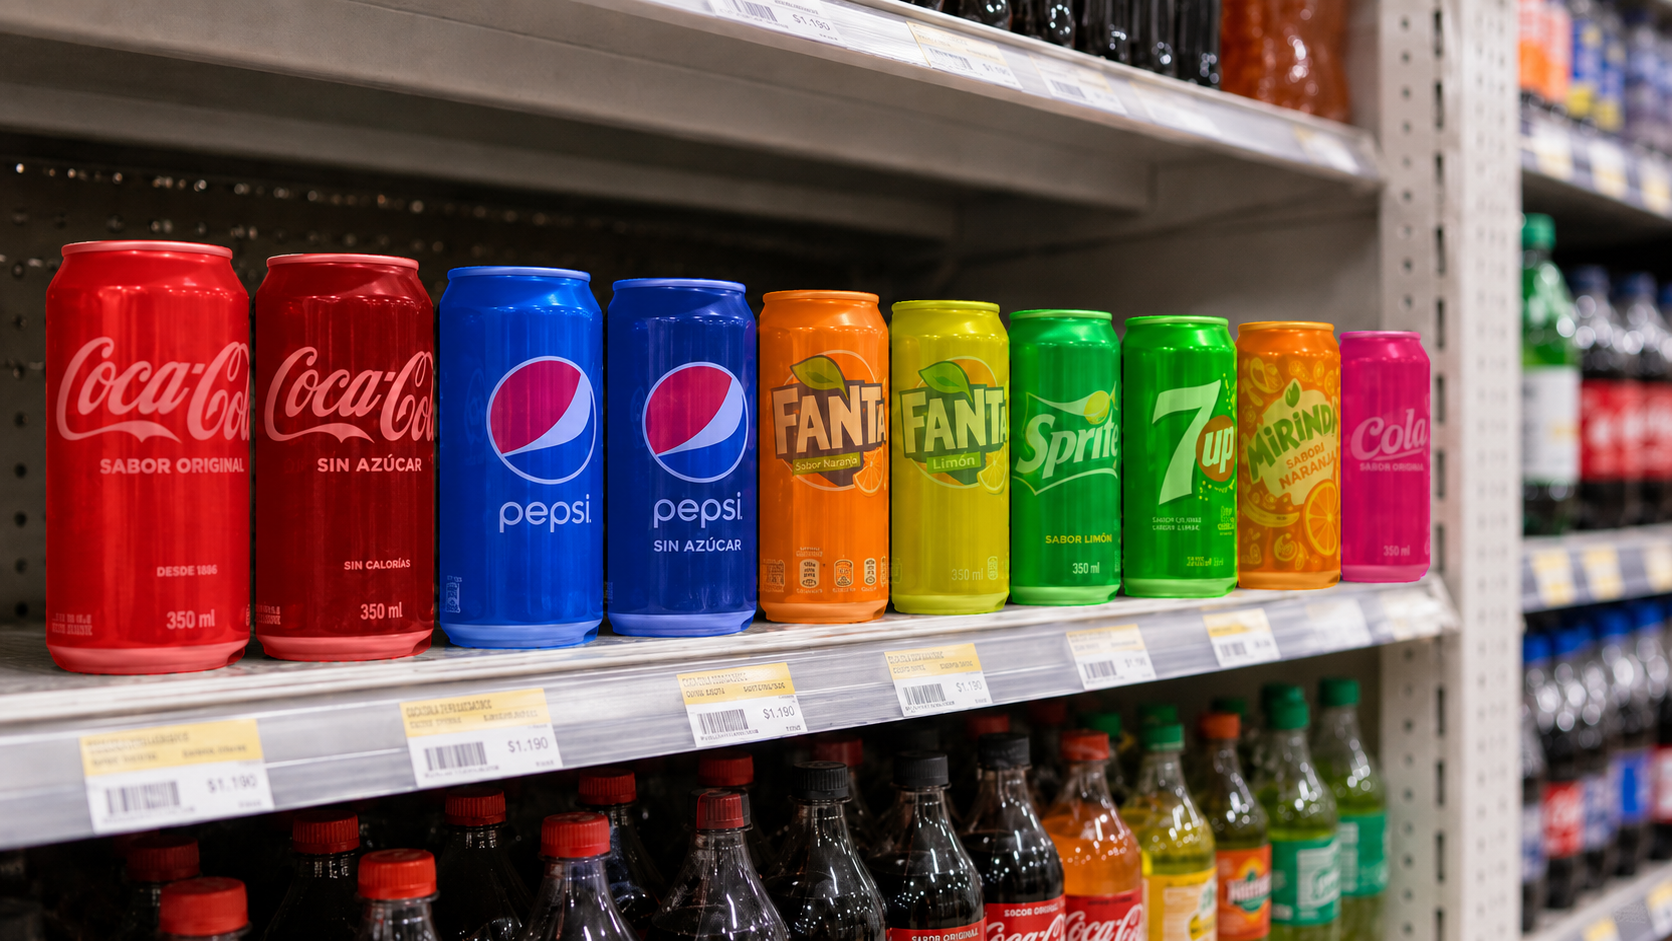
\includegraphics[width=0.78\textwidth]{fig_task_segmentation.png}
  \end{center}

  \vspace{4pt}
  {\footnotesize
  \begin{itemize}\setlength{\itemsep}{2pt}
    \item[{\color{arcaRed}\scriptsize\faArrowRight}]
      \textbf{Salida:} m\'ascara por \emph{pixel} (cada pixel etiquetado).
    \item[{\color{arcaRed}\scriptsize\faArrowRight}]
      M\'as costoso de etiquetar y entrenar, pero precisi\'on al pixel.
    \item[{\color{arcaRed}\scriptsize\faArrowRight}]
      Casos: medicina (delimitar tumor), agricultura (\'area cultivada).
  \end{itemize}
  }
\end{frame}

\begin{frame}[shrink]{4. Pose / Keypoints}
  \vspace{4pt}
  \begin{center}
    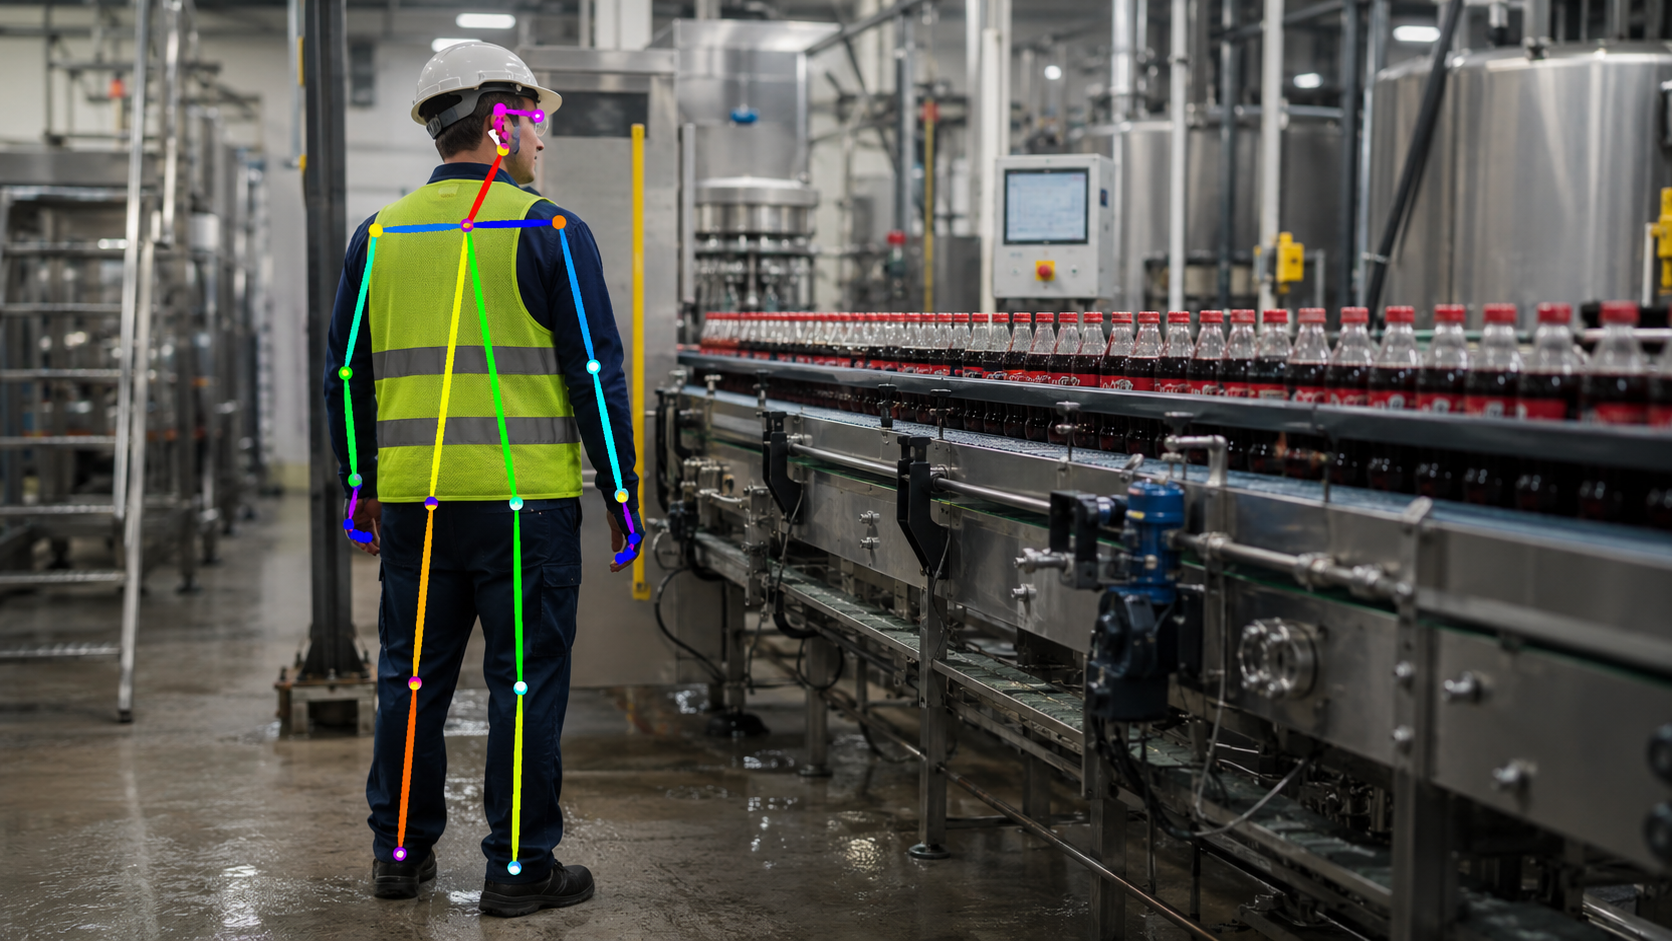
\includegraphics[width=0.78\textwidth]{fig_task_pose.png}
  \end{center}

  \vspace{4pt}
  {\footnotesize
  \begin{itemize}\setlength{\itemsep}{2pt}
    \item[{\color{arcaRed}\scriptsize\faArrowRight}]
      \textbf{Salida:} puntos clave (articulaciones) conectados.
    \item[{\color{arcaRed}\scriptsize\faArrowRight}]
      Casos: an\'alisis deportivo, ergonom\'ia, vigilancia de movimientos.
  \end{itemize}
  }
\end{frame}

\begin{frame}[shrink]{5. OCR (lectura de texto)}
  \vspace{4pt}
  \begin{center}
    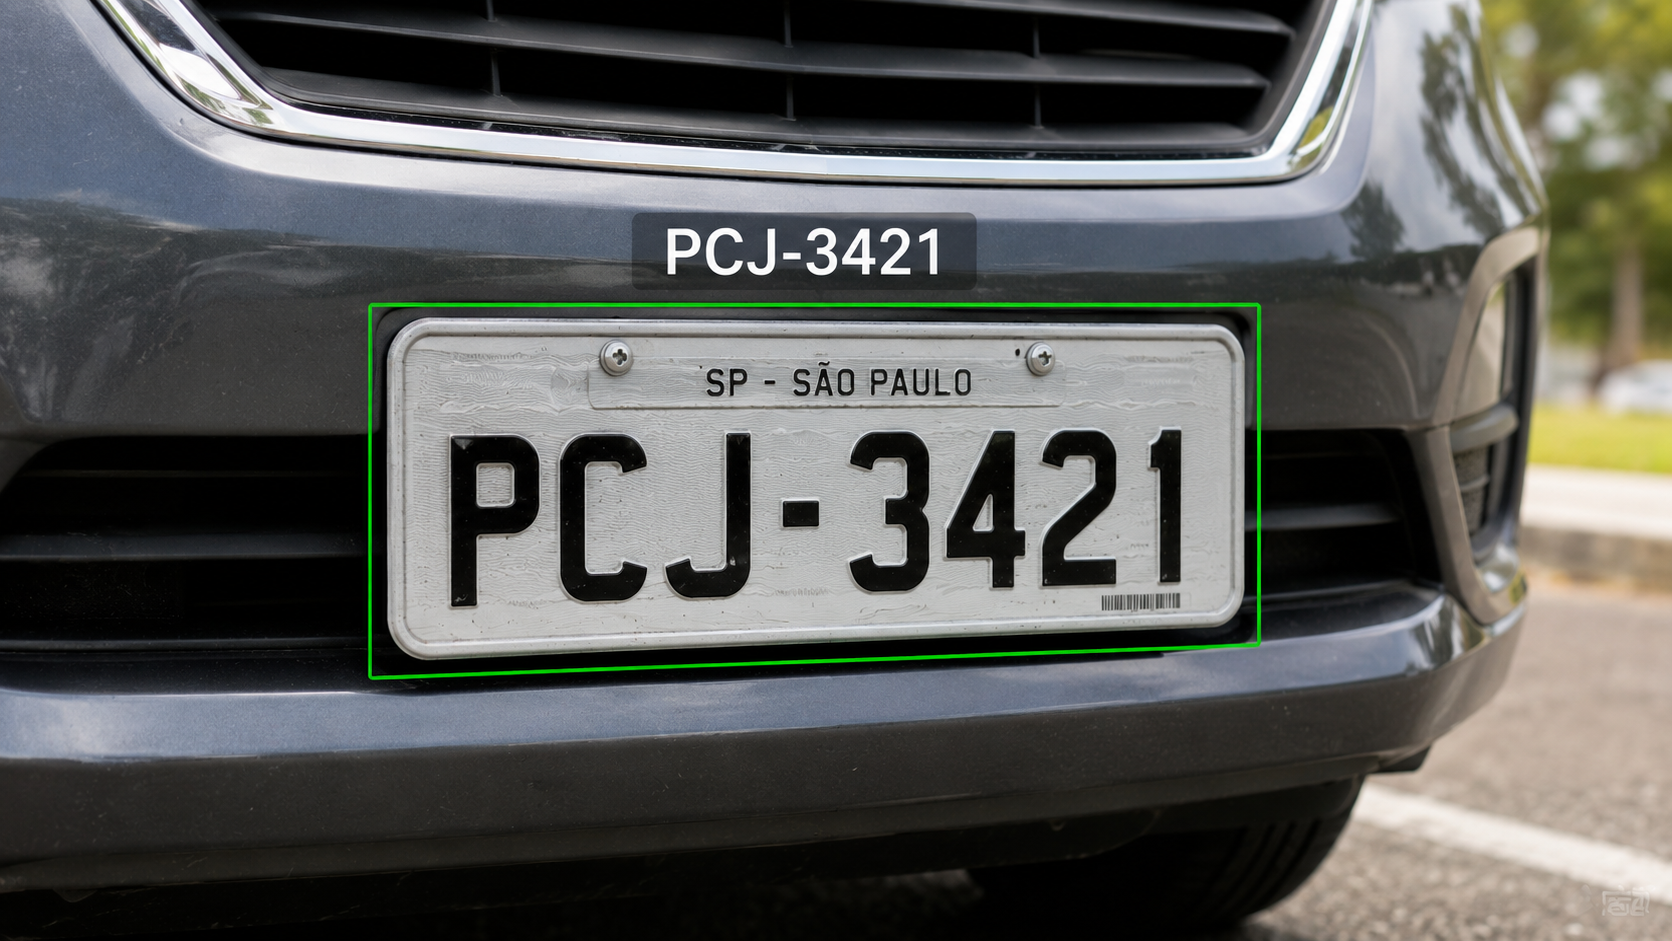
\includegraphics[width=0.78\textwidth]{fig_task_ocr.png}
  \end{center}

  \vspace{4pt}
  {\footnotesize
  \begin{itemize}\setlength{\itemsep}{2pt}
    \item[{\color{arcaRed}\scriptsize\faArrowRight}]
      \textbf{Salida:} la cadena de texto extra\'ida.
    \item[{\color{arcaRed}\scriptsize\faArrowRight}]
      Casos: lectura de placas, fechas de vencimiento, lotes, recibos.
    \item[{\color{codeGreen}\scriptsize\faArrowRight}]
      Suele combinarse con detecci\'on: detectar el rect\'angulo $\to$ leer el texto adentro.
  \end{itemize}
  }
\end{frame}

\begin{frame}[shrink]{?`Cu\'al Tarea Para Cu\'al Problema?}
  \vspace{8pt}
  {\footnotesize
  \begin{tabular}{@{}p{6.0cm} p{6.5cm}@{}}
    \toprule
    \textbf{Si tu pregunta es\ldots} & \textbf{La tarea es\ldots} \\
    \midrule
    \rowcolor{arcaGray}
    ?`Esta lata est\'a defectuosa? (1 producto por foto)
    & Clasificaci\'on \\
    ?`Cu\'antas latas hay en la g\'ondola y de qu\'e marca?
    & Detecci\'on \\
    \rowcolor{arcaGray}
    ?`Qu\'e \'area de la cinta transportadora ocupa el producto?
    & Segmentaci\'on \\
    ?`El operario tiene la mano cerca de zona peligrosa?
    & Pose / keypoints \\
    \rowcolor{arcaGray}
    ?`Cu\'al es el c\'odigo de lote impreso en esta caja?
    & OCR \\
    ?`Qu\'e dice la placa del cami\'on que ingresa?
    & \textbf{Detecci\'on + OCR (cascada)} \\
    \bottomrule
  \end{tabular}
  }

  \vspace{14pt}
  \begin{tcolorbox}[colback=arcaGray, colframe=arcaRed, boxrule=0.5pt,
    arc=2pt, left=6pt, right=6pt, top=4pt, bottom=4pt]
    {\scriptsize\color{arcaDark}
    \faKey\hspace{4pt}\textbf{Hoy nos enfocamos en detecci\'on}: c\'omo
    salir de ``una respuesta por imagen'' a ``N respuestas con su ubicaci\'on''.}
  \end{tcolorbox}
\end{frame}

% =============================================================================
%  BLOQUE E: BOUNDING BOXES + IoU
% =============================================================================
\sectionframe{Bounding Boxes e IoU}{La gram\'atica de la detecci\'on}

\begin{frame}[shrink]{Anatom\'ia de un Bounding Box}
  \vspace{4pt}
  \begin{center}
    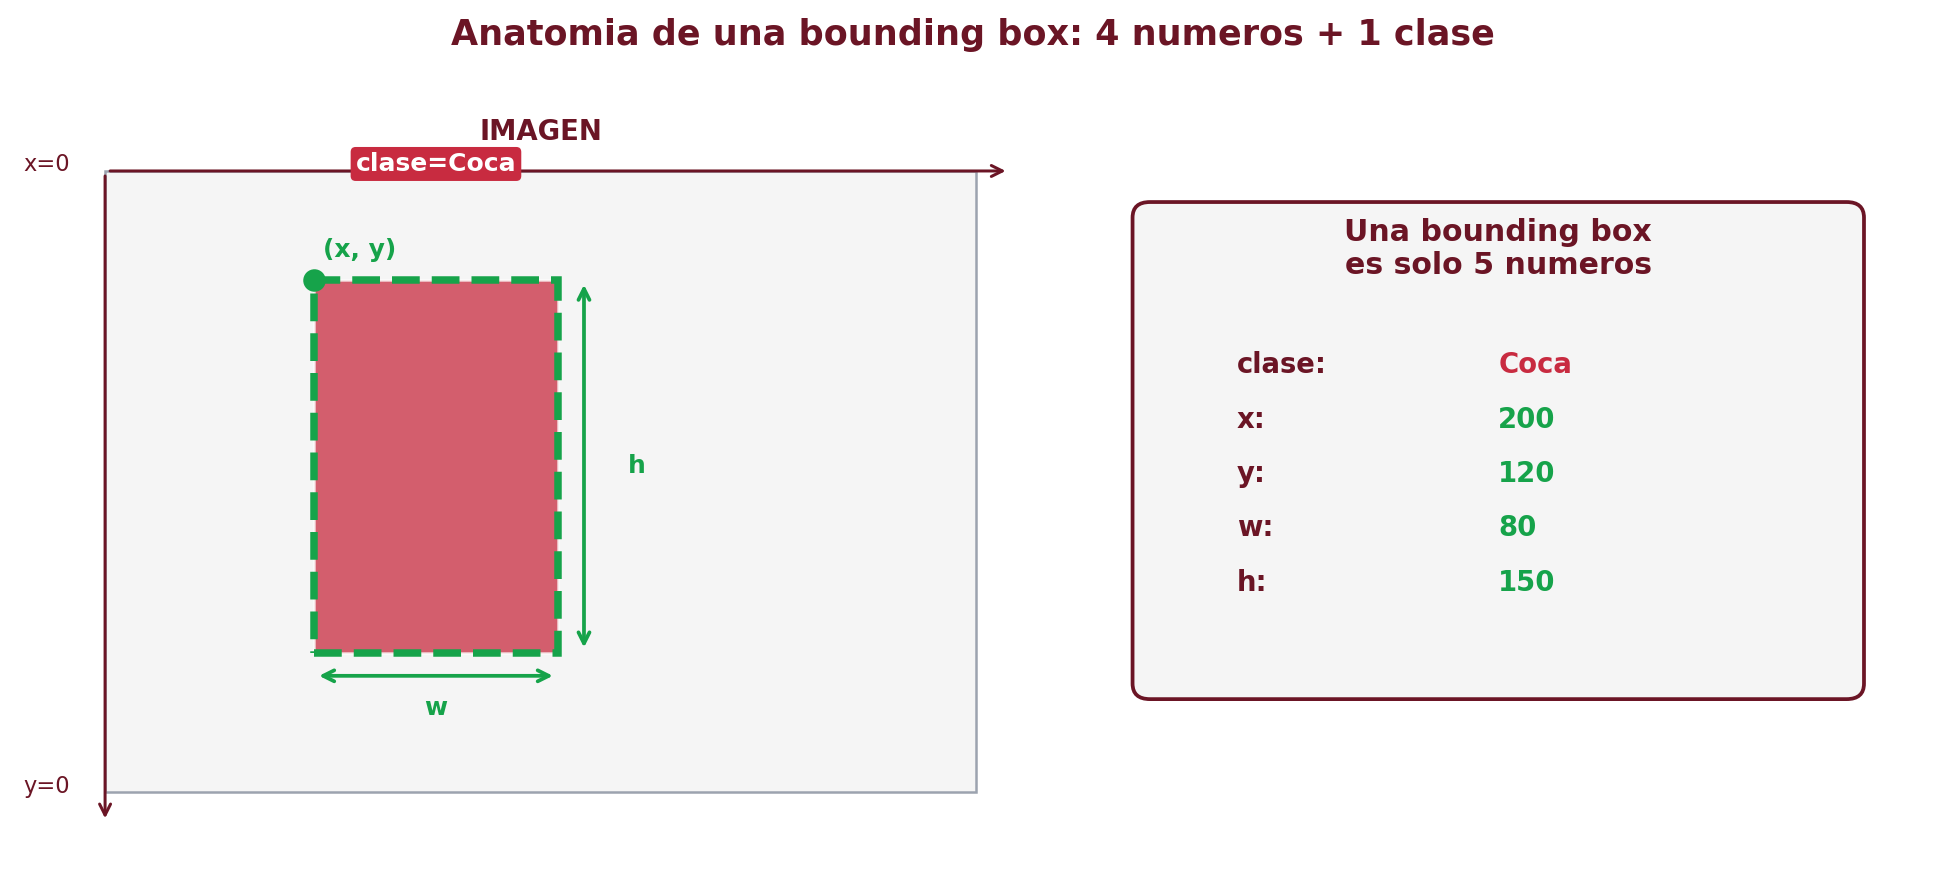
\includegraphics[width=0.95\textwidth]{fig_bbox.png}
  \end{center}

  \vspace{4pt}
  {\scriptsize\color{textMuted}
    \faLightbulb\hspace{4pt} Un bbox = (\textbf{x, y, w, h, clase}).
    Es la unidad b\'asica de la detecci\'on: cada objeto encontrado
    se reporta como un rect\'angulo con su etiqueta.}
\end{frame}

\begin{frame}[shrink]{IoU: ?`Qu\'e Tan Buena Es Una Predicci\'on?}
  \vspace{4pt}
  {\footnotesize\color{arcaDark}\bfseries
    \textbf{IoU} (Intersection over Union) compara la caja real con la
    predicha: $\text{IoU} = \dfrac{\text{intersecci\'on}}{\text{uni\'on}}$. Va de 0 a 1.}

  \vspace{6pt}
  \begin{center}
    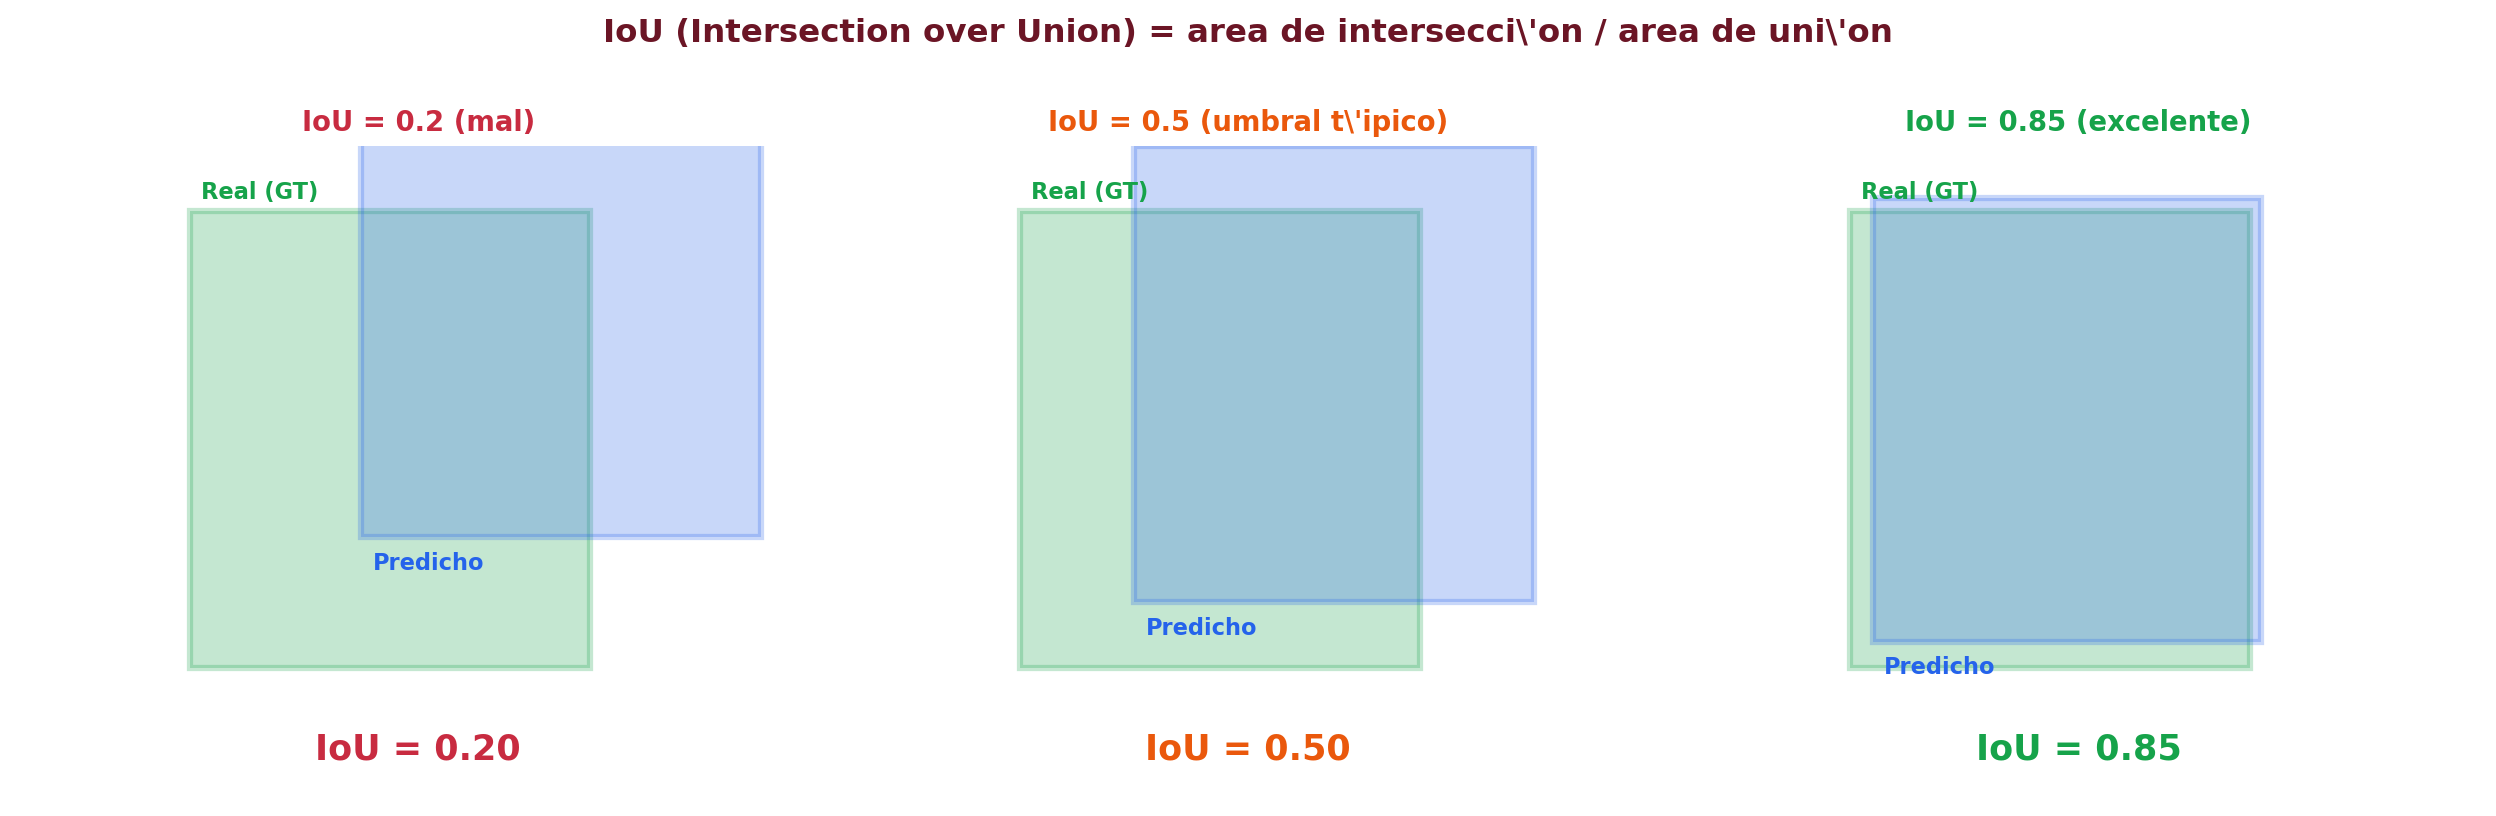
\includegraphics[width=0.95\textwidth]{fig_iou.png}
  \end{center}

  \vspace{2pt}
  {\scriptsize\color{textMuted}
    \faLightbulb\hspace{4pt} Convenci\'on: IoU $\geq$ 0.5 cuenta como
    detecci\'on correcta. Volveremos a esto cuando hablemos de m\'etricas.}
\end{frame}

% =============================================================================
%  BLOQUE F: APP 1 --- SLIDING WINDOW (NUEVO)
% =============================================================================

% =============================================================================
%  MULTI-OUTPUT — como una CNN puede predecir 5 numeros
% =============================================================================
\sectionframe{De Clasificaci\'on a Detecci\'on}{?`C\'omo predice una red 5 n\'umeros a la vez?}

\begin{frame}[shrink]{Recordemos: La Salida de una CNN Cl\'asica}
  \vspace{8pt}
  {\footnotesize\color{arcaDark}\bfseries
    Hasta ahora nuestras CNN dan \textbf{un solo n\'umero / vector} como salida:
    la probabilidad de cada clase. Pero un bbox necesita \textbf{5 n\'umeros}:
    x, y, w, h, clase. ?`C\'omo funciona eso?}

  \vspace{14pt}
  {\footnotesize
  \begin{itemize}\setlength{\itemsep}{6pt}
    \item[{\color{arcaRed}\scriptsize\faArrowRight}]
      Clasificaci\'on binaria: \texttt{Dense(1, sigmoid)} $\to$ 1 n\'umero (probabilidad).
    \item[{\color{arcaRed}\scriptsize\faArrowRight}]
      Clasificaci\'on multi-clase: \texttt{Dense(N, softmax)} $\to$ N probabilidades.
    \item[{\color{arcaRed}\scriptsize\faArrowRight}]
      Regresi\'on: \texttt{Dense(1)} (sin softmax) $\to$ un n\'umero continuo.
    \item[{\color{codeGreen}\scriptsize\faArrowRight}]
      \textbf{?`Y si queremos varios n\'umeros distintos al mismo tiempo?}
  \end{itemize}
  }
\end{frame}

\begin{frame}[shrink]{Multi-Output: 5 Cabezas Paralelas}
  \vspace{4pt}
  \begin{center}
    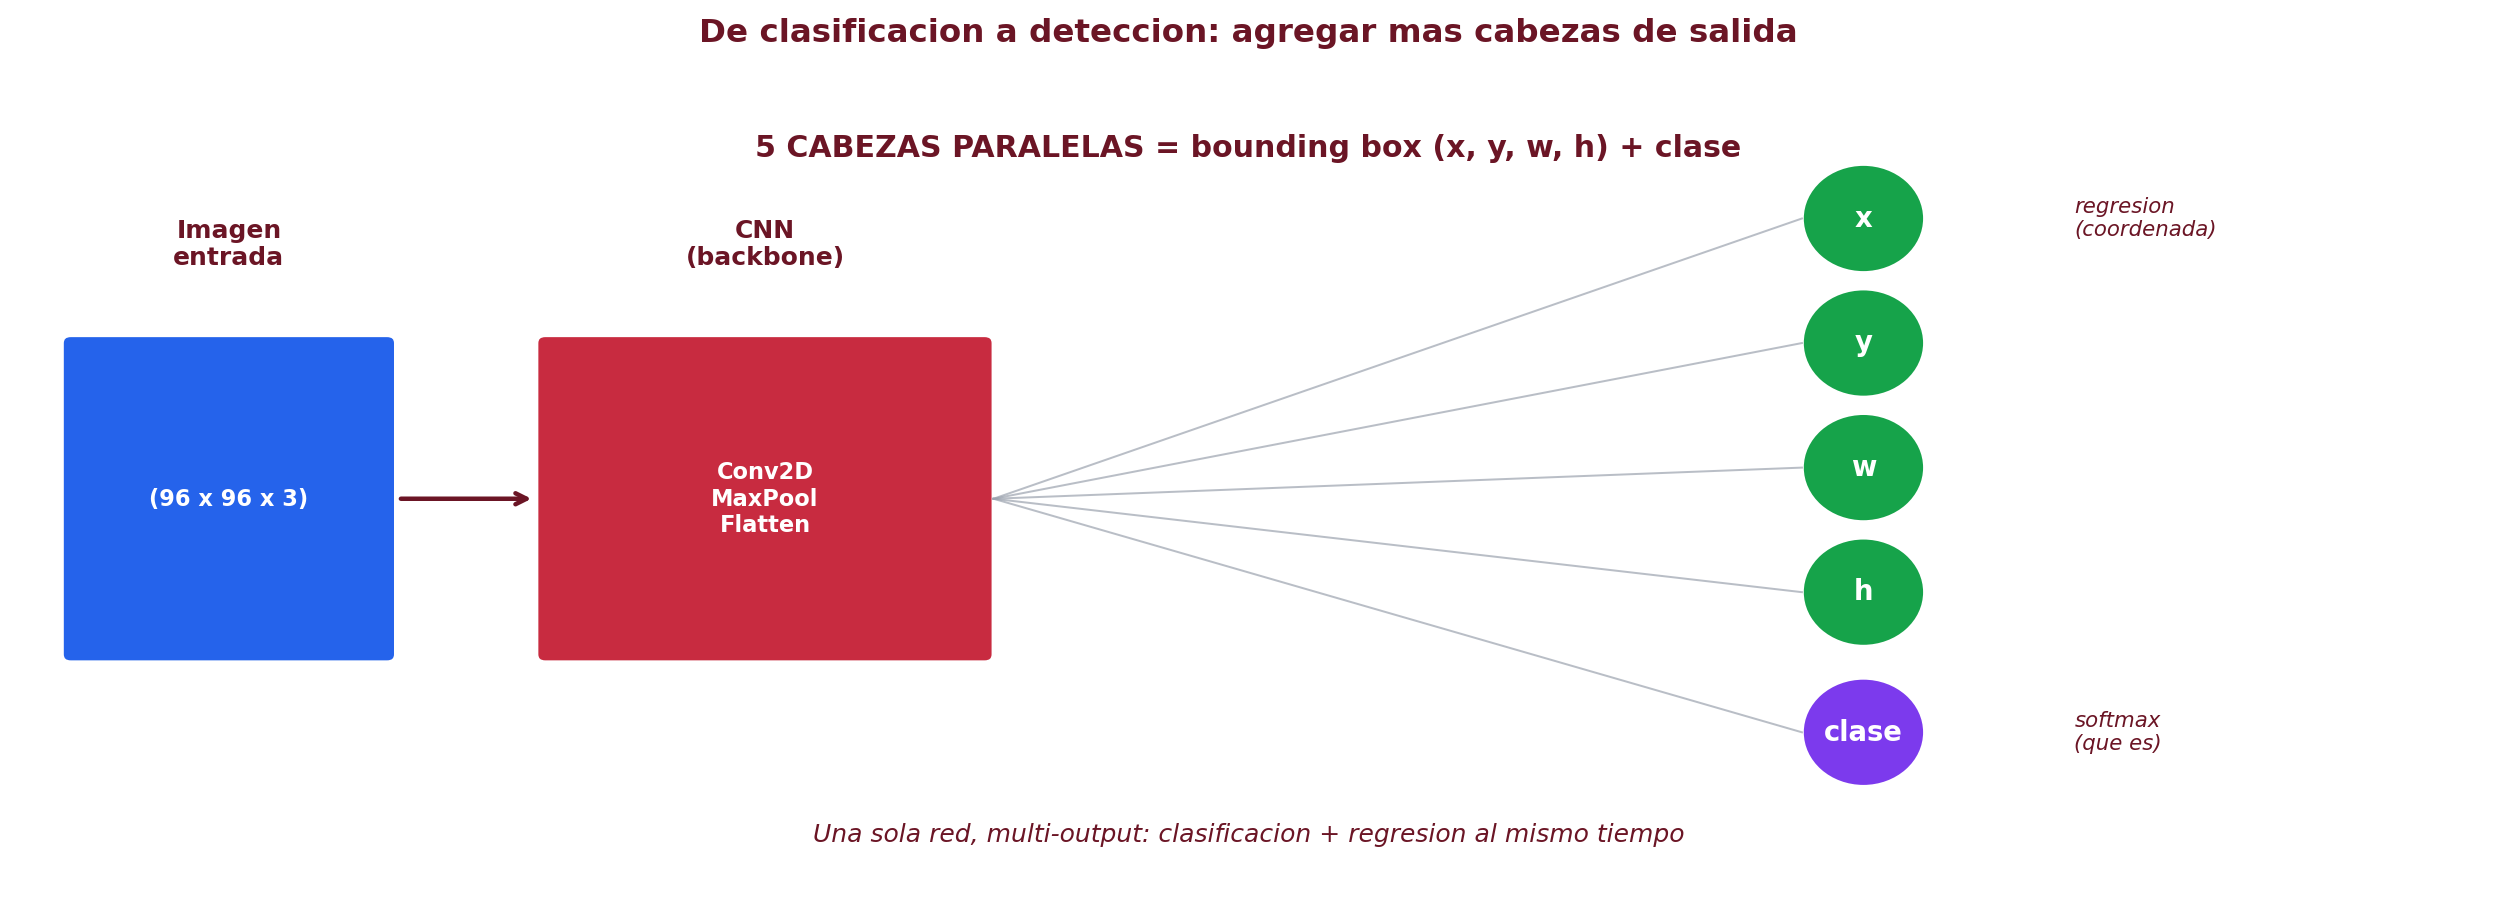
\includegraphics[width=0.95\textwidth]{fig_multioutput.png}
  \end{center}

  \vspace{4pt}
  {\scriptsize\color{textMuted}
    \faLightbulb\hspace{4pt} Una sola CNN comparte el backbone, pero
    \textbf{5 capas Dense paralelas} predicen las 5 salidas. 4 de regresi\'on
    (coordenadas) + 1 de clasificaci\'on (qu\'e clase). El optimizador
    entrena todas a la vez.}
\end{frame}

\begin{frame}[fragile,shrink]{C\'odigo: Red Multi-Output en Keras}
  \vspace{-4pt}
  \begin{pyblock}
from tensorflow.keras import layers, Model

inp = layers.Input(shape=(96, 96, 3))
x = layers.Conv2D(32, 3, activation="relu")(inp)
x = layers.MaxPooling2D()(x)
x = layers.Conv2D(64, 3, activation="relu")(x)
x = layers.MaxPooling2D()(x)
x = layers.Flatten()(x)
x = layers.Dense(64, activation="relu")(x)

# 5 CABEZAS PARALELAS
out_x = layers.Dense(1, name="x")(x)
out_y = layers.Dense(1, name="y")(x)
out_w = layers.Dense(1, name="w")(x)
out_h = layers.Dense(1, name="h")(x)
out_cls = layers.Dense(2, activation="softmax", name="clase")(x)

model = Model(inp, [out_x, out_y, out_w, out_h, out_cls])
model.compile(optimizer="adam",
              loss=["mse","mse","mse","mse","sparse_categorical_crossentropy"])
  \end{pyblock}
\end{frame}

\begin{frame}[shrink]{?`Y Si Hay Varios Objetos en una Imagen?}
  \vspace{8pt}
  {\footnotesize\color{arcaDark}\bfseries
    Este multi-output funciona para \textbf{un objeto} por imagen.
    ?`Y si hay 5 carros con 5 placas distintas?}

  \vspace{14pt}
  {\footnotesize
  \begin{itemize}\setlength{\itemsep}{6pt}
    \item[{\color{arcaRed}\scriptsize\faArrowRight}]
      Una salida fija no puede manejar cantidad variable de objetos.
    \item[{\color{arcaRed}\scriptsize\faArrowRight}]
      \textbf{Idea ingenua \#1}: barrer la imagen con un clasificador
      (\emph{sliding window}). Vamos a verlo en la siguiente secci\'on.
    \item[{\color{arcaRed}\scriptsize\faArrowRight}]
      \textbf{Idea ingenua \#2}: predecir 100 bboxes fijos. Mayor\'ia ser\'an
      vac\'ios, hay que filtrar.
    \item[{\color{codeGreen}\scriptsize\faArrowRight}]
      \textbf{Idea elegante (YOLO)}: una sola CNN cuya salida es un
      tensor con grilla espacial; en cada posici\'on del tensor sale
      un set de outputs $(x,y,w,h,\text{clase})$. Lo vemos despu\'es.
  \end{itemize}
  }
\end{frame}


\begin{frame}[shrink]{Sliding Window: La Idea Ingenua (y Por Qu\'e No Sirve)}
  \vspace{8pt}
  {\footnotesize\color{arcaDark}\bfseries
    \textbf{Idea naive:} recorrer la imagen con una ventana clasificadora
    en cada posici\'on, y guardar las cajas que pasen el umbral.}

  \vspace{14pt}
  {\footnotesize
  \begin{tabular}{@{}p{6.0cm} r@{}}
    \toprule
    \textbf{Caso} & \textbf{Pasadas necesarias} \\
    \midrule
    \rowcolor{arcaGray}
    Imagen 96$\times$96, ventana 16, stride 8
    & $\sim$120 \\
    Imagen 640$\times$640, ventana 32, stride 4
    & $\sim$25\,000 \\
    \rowcolor{arcaGray}
    Igual + 3 escalas distintas de ventana
    & $\sim$75\,000 \\
    \midrule
    A 1ms por pasada en GPU r\'apida
    & $\sim$\textbf{75 segundos por imagen} \\
    \bottomrule
  \end{tabular}
  }

  \vspace{14pt}
  \begin{tcolorbox}[colback=arcaRed!8, colframe=arcaRed, boxrule=0.5pt,
    arc=2pt, left=6pt, right=6pt, top=4pt, bottom=4pt]
    {\scriptsize\color{arcaDark}
    \faExclamationTriangle\hspace{4pt} \textbf{Inviable.} Hace falta una
    arquitectura que produzca \textbf{m\'ultiples bboxes en una sola pasada}.
    Esa es la idea de \textbf{YOLO} --- al grano.}
  \end{tcolorbox}
\end{frame}

% =============================================================================
%  BLOQUE G: YOLO EN PROFUNDIDAD
% =============================================================================
\sectionframe{C\'omo Funciona YOLO}{La idea revolucionaria de 2015}

\begin{frame}[shrink]{La Idea: ``You Only Look Once''}
  \vspace{6pt}
  {\footnotesize\color{arcaDark}\bfseries
    Antes de YOLO los detectores hac\'ian dos pasadas: primero buscar
    regiones de inter\'es, despu\'es clasificar cada una. \textbf{Lento}.
    YOLO lo hace todo \textbf{de un solo tir\'on}.}

  \vspace{14pt}
  {\footnotesize
  \begin{itemize}\setlength{\itemsep}{8pt}
    \item[{\color{arcaRed}\scriptsize\faArrowRight}]
      Le pasas la imagen completa a la red \textbf{una sola vez}.
    \item[{\color{arcaRed}\scriptsize\faArrowRight}]
      La red devuelve directamente una \textbf{lista de cajas}: cada caja
      con sus coordenadas, su clase y qu\'e tan segura est\'a.
    \item[{\color{arcaRed}\scriptsize\faArrowRight}]
      Como la red est\'a entrenada para mirar la imagen ``por pedazos''
      al mismo tiempo, puede detectar varios objetos a la vez.
    \item[{\color{codeGreen}\scriptsize\faArrowRight}]
      Al final pasa por un filtro (\textbf{NMS}) que elimina cajas
      repetidas y deja una por objeto.
  \end{itemize}
  }
\end{frame}

\begin{frame}[shrink]{La Rejilla, Visualmente}
  \vspace{4pt}
  \begin{center}
    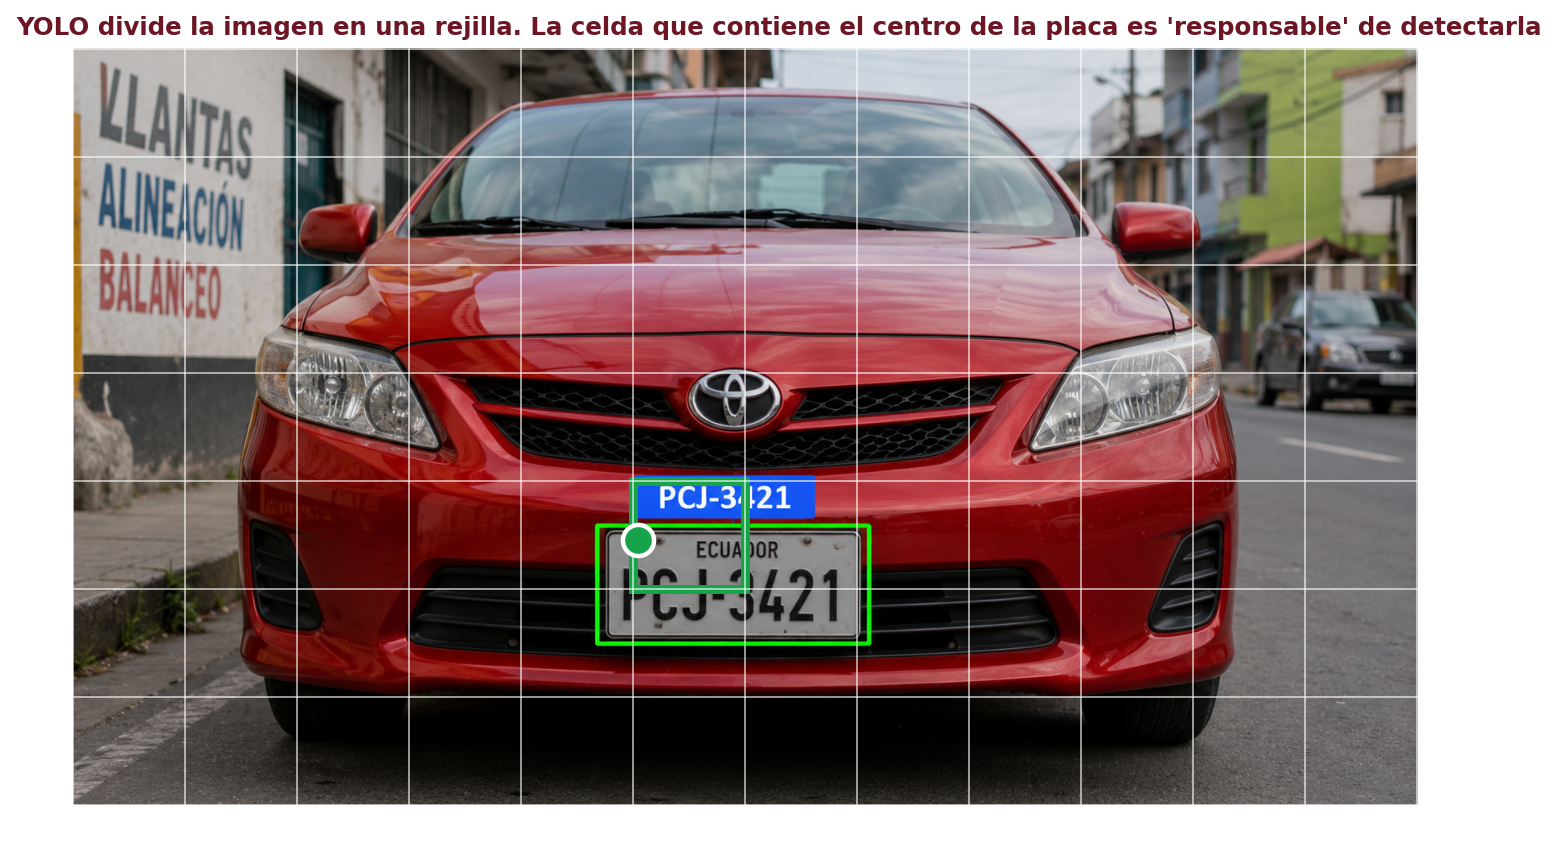
\includegraphics[width=0.85\textwidth]{fig_yolo_grid.png}
  \end{center}

  \vspace{4pt}
  {\scriptsize\color{textMuted}
    \faLightbulb\hspace{4pt} Imag\'inate que la imagen queda dividida en
    una cuadr\'icula invisible. La red entrega muchas cajas en paralelo
    (una por zona) y despu\'es se queda con las mejores.
    En YOLO26 hay 3 cuadr\'iculas de distinto tama\~no para detectar
    objetos peque\~nos y grandes al tiempo.}
\end{frame}

\begin{frame}[shrink]{NMS: Limpiar Detecciones Duplicadas}
  \vspace{4pt}
  {\footnotesize\color{arcaDark}\bfseries
    YOLO produce \textbf{cientos} de detecciones por imagen, varias
    del mismo objeto. \textbf{NMS} (Non-Maximum Suppression) deja una sola.}

  \vspace{6pt}
  \begin{center}
    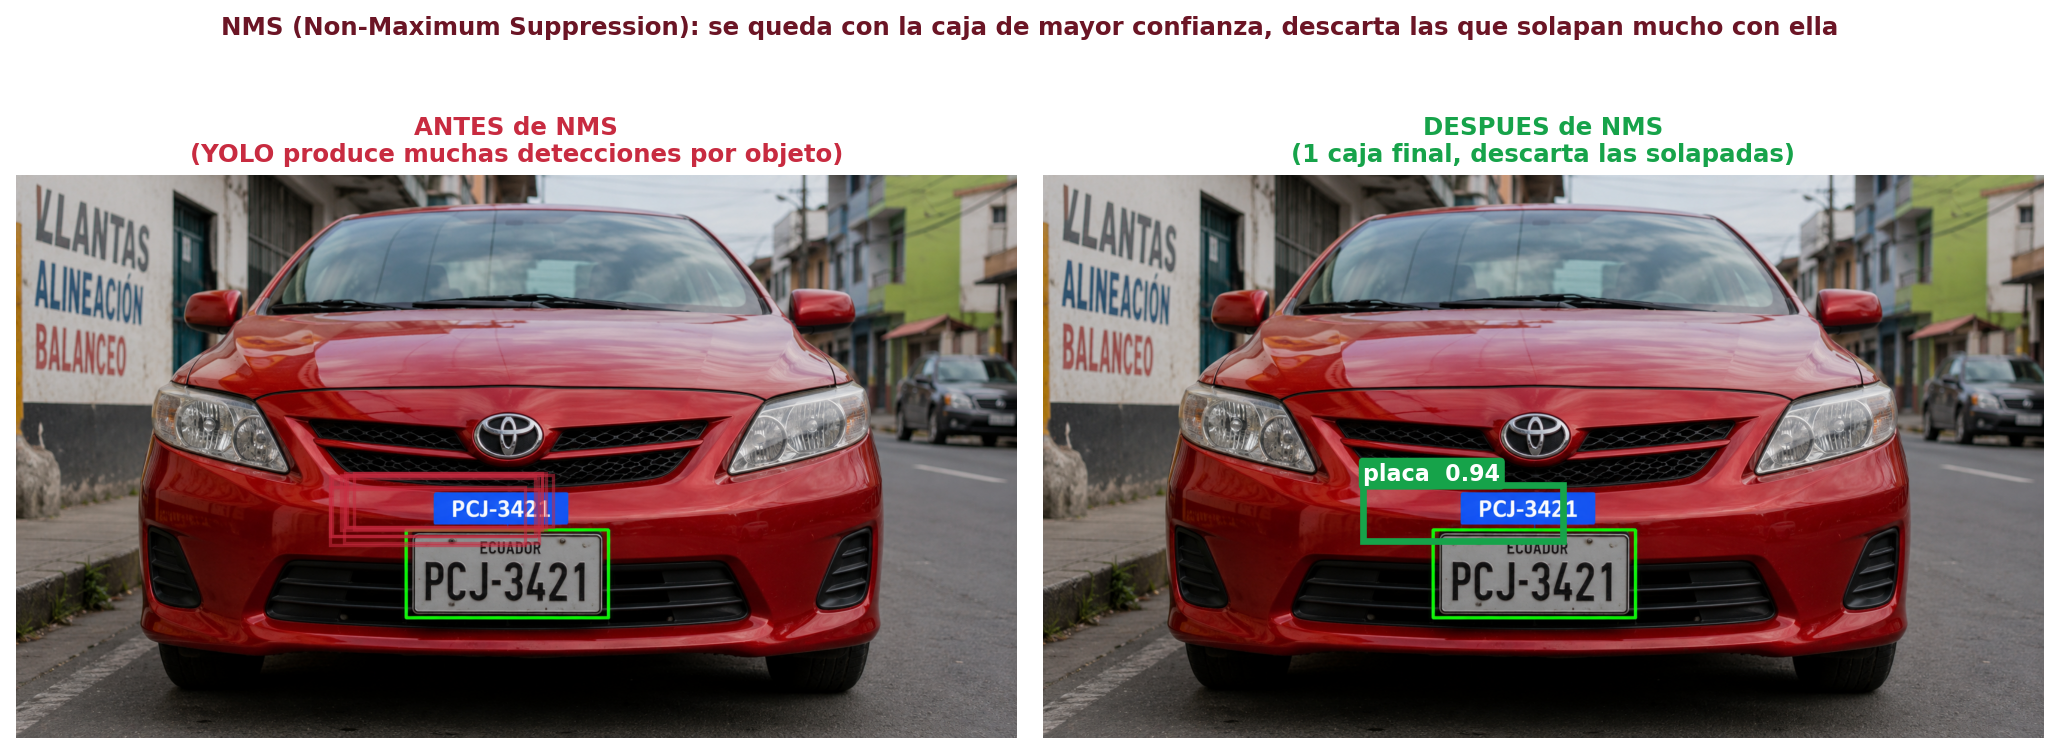
\includegraphics[width=0.95\textwidth]{fig_nms.png}
  \end{center}

  \vspace{2pt}
  {\scriptsize\color{textMuted}
    \faLightbulb\hspace{4pt} Algoritmo: ordenar por confianza, quedarse
    con la mejor, descartar las que solapan con IoU $>$ 0.5. Repetir.
    Lo mismo que el sliding window deber\'ia haber hecho.}
\end{frame}

\begin{frame}[shrink]{Una D\'ecada de YOLO}
  \vspace{4pt}
  \begin{center}
    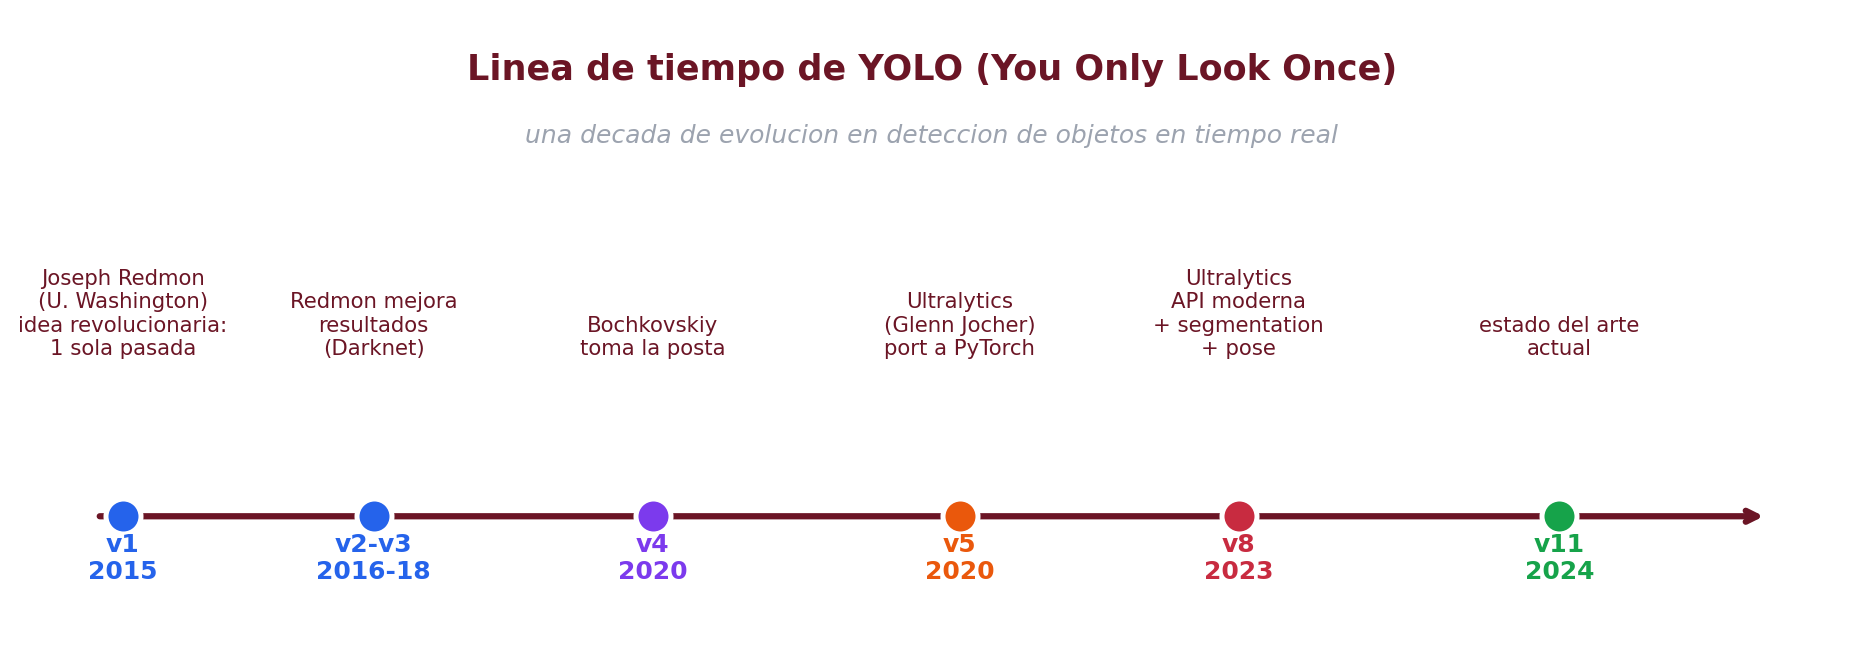
\includegraphics[width=0.97\textwidth]{fig_yolo_timeline.png}
  \end{center}

  \vspace{6pt}
  {\scriptsize
  \begin{itemize}\setlength{\itemsep}{2pt}
    \item[{\color{arcaRed}\scriptsize\faArrowRight}]
      \textbf{Joseph Redmon (v1, 2015):} idea original, paper famoso.
      Framework Darknet en C.
    \item[{\color{arcaRed}\scriptsize\faArrowRight}]
      \textbf{Bochkovskiy (v4, 2020):} continu\'o cuando Redmon abandon\'o.
    \item[{\color{arcaRed}\scriptsize\faArrowRight}]
      \textbf{Ultralytics (v5+, 2020+):} port a PyTorch, API moderna.
    \item[{\color{codeGreen}\scriptsize\faArrowRight}]
      \textbf{YOLO26 (Ultralytics, ene 2026):} \'ultima versi\'on,
      es la que vamos a usar.
  \end{itemize}
  }
\end{frame}

\begin{frame}[shrink]{La Familia: Velocidad vs Precisi\'on}
  \vspace{4pt}
  \begin{center}
    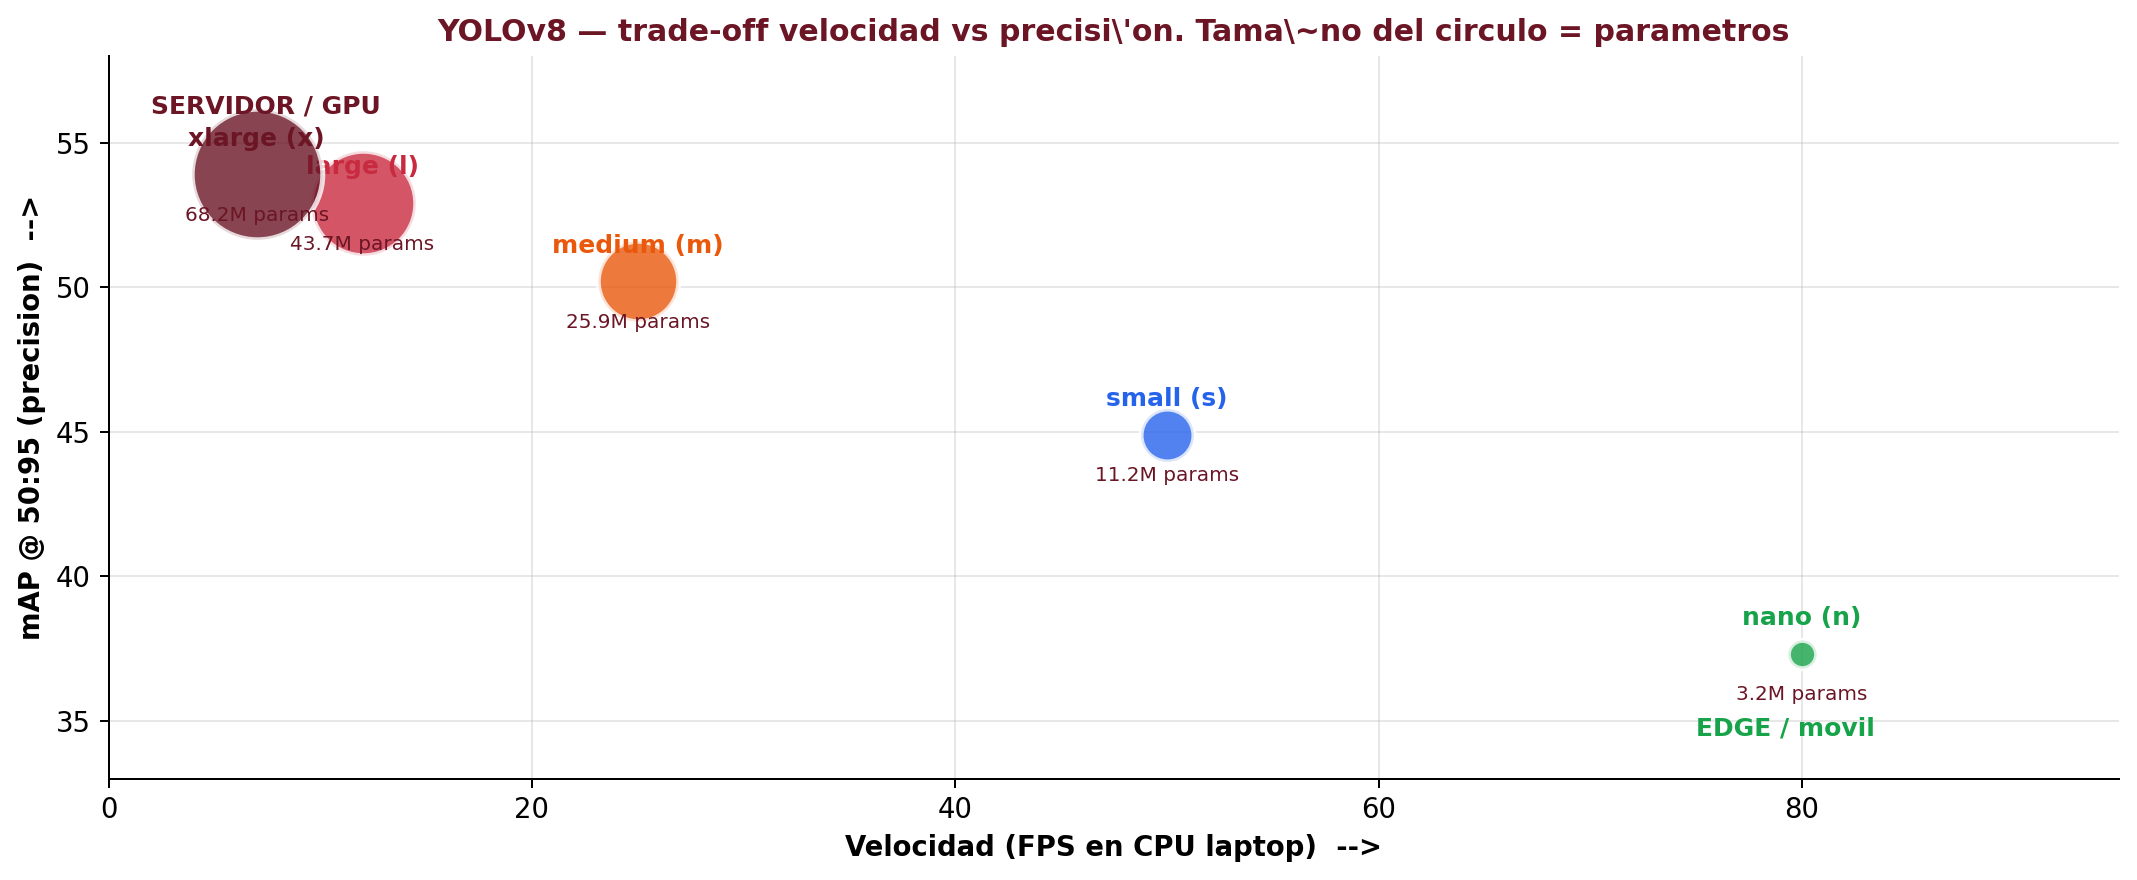
\includegraphics[width=0.92\textwidth]{fig_yolo_family.png}
  \end{center}

  \vspace{4pt}
  {\scriptsize\color{textMuted}
    \faLightbulb\hspace{4pt} 5 tama\~nos (n, s, m, l, x): la \emph{misma}
    arquitectura con distinta cantidad de filtros. M\'as filtros = m\'as
    preciso pero m\'as lento.}
\end{frame}

\begin{frame}[shrink]{?`Cu\'al Modelo Eligir?}
  \vspace{8pt}
  {\footnotesize
  \begin{tabular}{@{}p{2.0cm} p{3.7cm} p{2.7cm} p{4.0cm}@{}}
    \toprule
    \textbf{Modelo} & \textbf{Hardware} & \textbf{Velocidad} & \textbf{Cu\'ando usarlo} \\
    \midrule
    \rowcolor{arcaGray}
    \textbf{nano (n)}  & CPU laptop, m\'ovil & 80+ FPS & Edge, IoT, c\'amara en vivo \\
    small (s)  & CPU buena o GPU peque\~na & 50 FPS & Demo r\'apido, prototipo \\
    \rowcolor{arcaGray}
    medium (m) & GPU consumer & 25 FPS & Producci\'on con buen hardware \\
    large (l)  & GPU dedicada & 12 FPS & Calidad alta, no tiempo real \\
    \rowcolor{arcaGray}
    xlarge (x) & GPU servidor & 7 FPS & M\'axima precisi\'on, batch off-line \\
    \bottomrule
  \end{tabular}
  }

  \vspace{14pt}
  \begin{tcolorbox}[colback=codeGreen!8, colframe=codeGreen, boxrule=0.5pt,
    arc=2pt, left=6pt, right=6pt, top=4pt, bottom=4pt]
    {\scriptsize\color{arcaDark}
    \faKey\hspace{4pt} Para nuestras pruebas y proyecto vamos con
    \textbf{YOLO26 nano}. Funciona en CPU de Colab y carga en segundos.}
  \end{tcolorbox}
\end{frame}

% =============================================================================
%  BLOQUE H: PROYECTO LPR + APP 2 YOLO PREENTRENADO
% =============================================================================
\sectionframe{Usar YOLO en C\'odigo}{El flujo normal: cargar, predecir, trabajar con resultados}

\begin{frame}[shrink]{El Proyecto que Viene: Lectura de Placas}
  \vspace{6pt}
  {\footnotesize\color{arcaDark}\bfseries
    Imaginen este caso real de Arca: control de acceso a planta.
    Cada cami\'on que entra debe registrarse en un libro --- un guardia
    anota la placa con bol\'igrafo. Lento, propenso a errores.}

  \vspace{6pt}
  \begin{center}
    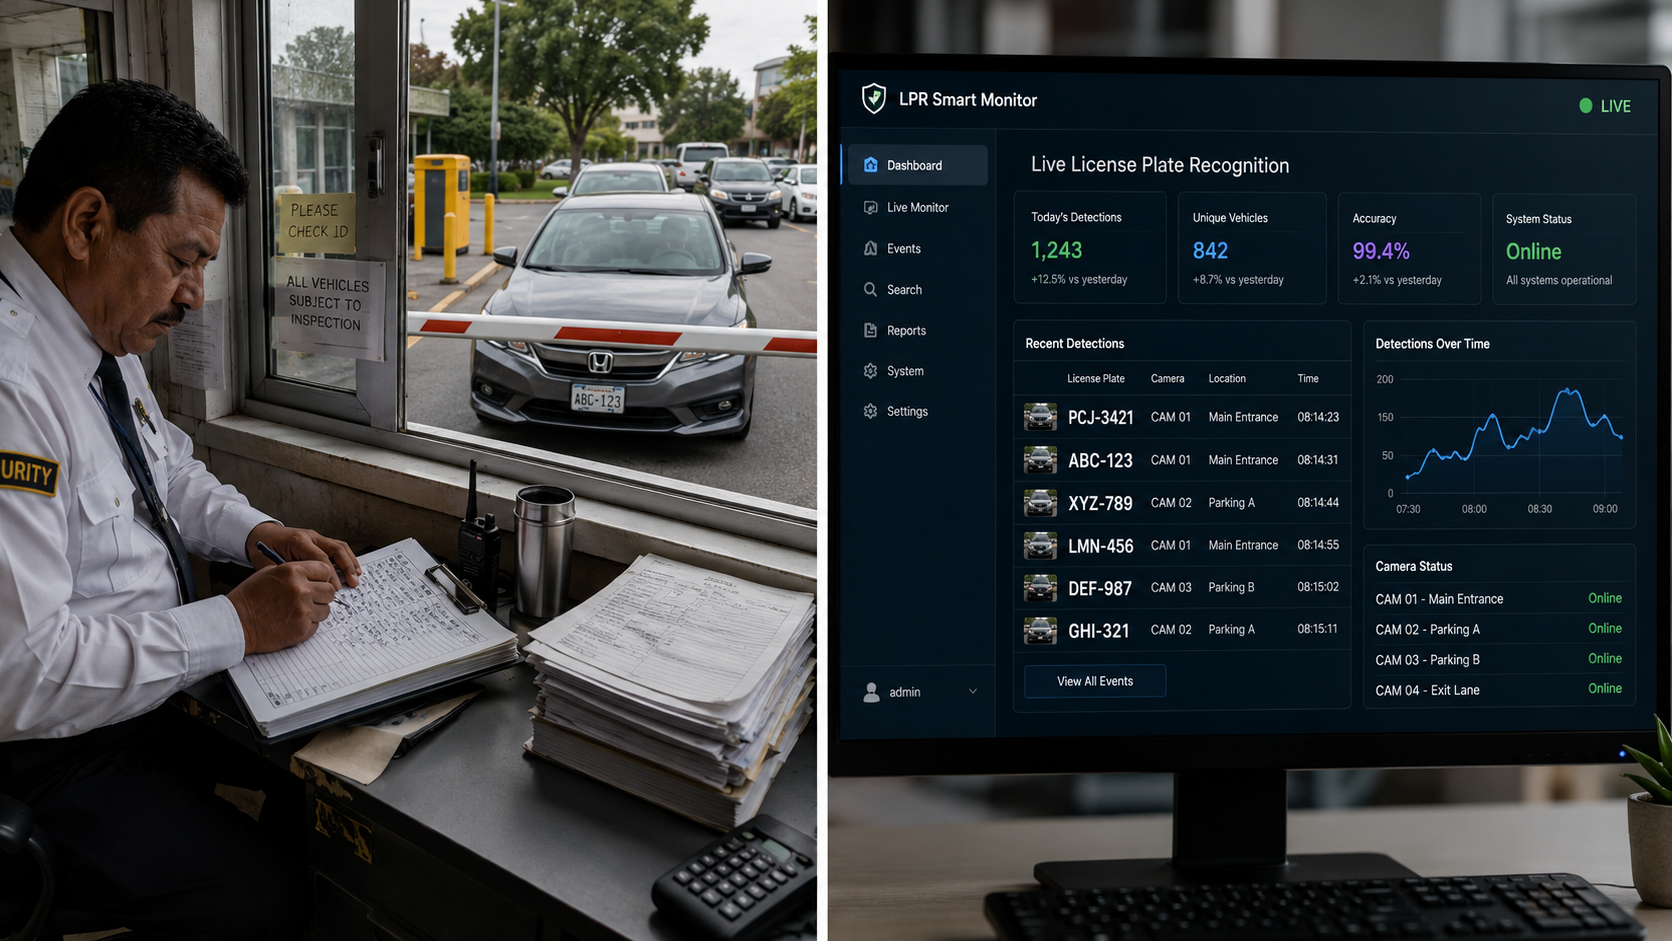
\includegraphics[width=0.55\textwidth]{fig_motivacion_problema.png}
  \end{center}

  \vspace{2pt}
  {\scriptsize\color{textMuted}
    \faLightbulb\hspace{4pt} Antes de fine-tunear, aprendamos a usar YOLO
    como una herramienta cualquiera --- igual que \texttt{sklearn}.}
\end{frame}

\begin{frame}[fragile,shrink]{1. Cargar el Modelo (Cu\'al Eligir)}
  \vspace{-4pt}
  \begin{pyblock}
from ultralytics import YOLO

# Los 5 tamanos de YOLO26 (mismo patron en v8, v11, v12...)
# yolo26n.pt   3M params   CPU, edge, movil    (rapido, menos preciso)
# yolo26s.pt  11M
# yolo26m.pt  25M
# yolo26l.pt  43M
# yolo26x.pt  68M params   GPU servidor        (lento, mas preciso)

model = YOLO("yolo26n.pt")    # baja pesos solo la 1ra vez
print(model.names)             # las 80 clases preentrenadas (COCO)
  \end{pyblock}

  \vspace{4pt}
  {\scriptsize\color{textMuted}
    \faLightbulb\hspace{4pt} \textbf{Default razonable:} arrancar con
    \texttt{nano} para prototipar; si la precisi\'on no alcanza, subir
    a \texttt{small} o \texttt{medium}.}
\end{frame}

\begin{frame}[fragile,shrink]{2. Inferencia en Una L\'inea}
  \vspace{-4pt}
  \begin{pyblock}
# Funciona con URL, archivo local, ndarray o PIL Image
results = model("https://eje21.com.co/.../auto.jpg")

# `results` es lista (un item por imagen procesada)
res = results[0]

# Mostrar de inmediato
res.show()                    # abre ventana o devuelve PIL
img_anotada = res.plot()      # ndarray BGR con cajas dibujadas
res.save("salida.jpg")        # guardar con cajas

print(f"Detecciones: {len(res.boxes)}")
  \end{pyblock}

  \vspace{4pt}
  {\scriptsize\color{textMuted}
    \faLightbulb\hspace{4pt} Una sola pasada de CNN. En CPU laptop con
    \texttt{yolo26n}: $\sim$50ms por imagen. En GPU T4: $\sim$5ms.}
\end{frame}

\begin{frame}[shrink]{3. Los 5 Par\'ametros Que Importan}
  \vspace{6pt}
  {\footnotesize
  \begin{tabular}{@{}p{2.3cm} p{6.0cm} p{2.5cm}@{}}
    \toprule
    \textbf{Par\'ametro} & \textbf{Qu\'e controla} & \textbf{Default} \\
    \midrule
    \rowcolor{arcaGray}
    \texttt{conf}
    & Umbral de confianza (filtra cajas d\'ebiles)
    & 0.25 \\
    \texttt{iou}
    & Umbral NMS (cu\'an solapadas las cajas)
    & 0.7 \\
    \rowcolor{arcaGray}
    \texttt{imgsz}
    & Resoluci\'on al procesar (objetos peque\~nos pide m\'as)
    & 640 \\
    \texttt{classes}
    & Filtrar solo ciertas clases (\texttt{[2, 7]} = car, truck)
    & None \\
    \rowcolor{arcaGray}
    \texttt{device}
    & D\'onde correr: \texttt{cpu}, \texttt{cuda}, \texttt{mps}
    & auto \\
    \bottomrule
  \end{tabular}
  }

  \vspace{10pt}
  \begin{tcolorbox}[colback=arcaGray, colframe=arcaRed, boxrule=0.5pt,
    arc=2pt, left=6pt, right=6pt, top=4pt, bottom=4pt]
    {\scriptsize\color{arcaDark}
    \faKey\hspace{4pt}\textbf{Heur\'istica r\'apida:} si quieres menos
    falsos positivos $\to$ sube \texttt{conf}. Si quieres detectar
    objetos peque\~nos $\to$ sube \texttt{imgsz} a 1280.}
  \end{tcolorbox}
\end{frame}

\begin{frame}[fragile,shrink]{4. Trabajar con los Resultados}
  \vspace{-4pt}
  \begin{pyblock}
res = model("auto.jpg", conf=0.5)[0]

# Iterar sobre cada deteccion
for box in res.boxes:
    x1, y1, x2, y2 = box.xyxy[0].tolist()    # corners
    cx, cy, w, h = box.xywh[0].tolist()      # center + size
    cls_id = int(box.cls[0])
    conf = float(box.conf[0])
    nombre = res.names[cls_id]
    print(f"{nombre}: conf={conf:.2f}")

# Conteo rapido por clase
from collections import Counter
clases = [res.names[int(c)] for c in res.boxes.cls]
print(Counter(clases))
  \end{pyblock}
\end{frame}

\begin{frame}[fragile,shrink]{5. Inferencia Sobre Video}
  \vspace{-4pt}
  \begin{pyblock}
# Misma API: pasar un mp4 (local o URL) en vez de una imagen.
# Por default guarda un mp4 de salida con las cajas dibujadas.

results = model(
    "traffic.mp4",
    conf=0.4,
    classes=[2, 7],         # car, truck
    save=True,              # guarda video resultado
    project="runs", name="video_demo",
)

print(f"Frames procesados: {len(results)}")
# Output queda en: runs/video_demo/traffic.avi
  \end{pyblock}

  \vspace{4pt}
  {\scriptsize\color{textMuted}
    \faLightbulb\hspace{4pt} Para webcam en vivo: pasar \texttt{0} como
    fuente (\'indice de c\'amara) o el path a una RTSP de IP camera.
    Mismo c\'odigo.}
\end{frame}

\begin{frame}[shrink]{Resumen: la API de YOLO en 4 Pasos}
  \vspace{14pt}
  {\footnotesize\color{arcaDark}\bfseries\centering
  \begin{tabular}{@{}rl@{}}
    \textbf{1.} & Cargar:\quad     \texttt{model = YOLO("yolo26n.pt")} \\[6pt]
    \textbf{2.} & Inferir:\quad    \texttt{results = model(source)} \\[6pt]
    \textbf{3.} & Desempacar:\quad \texttt{res = results[0]} \\[6pt]
    \textbf{4.} & Usar:\quad       \texttt{res.plot(); res.boxes; res.save()}
  \end{tabular}
  }

  \vspace{14pt}
  {\footnotesize
    Eso es \textbf{todo} lo que necesitan para usar YOLO en sus proyectos.
    Funciona para im\'agenes, videos, streams de webcam y URLs. La API es
    la misma.}
\end{frame}

\begin{frame}[shrink]{Experimento: Suban Una Foto con una Placa}
  \vspace{6pt}
  {\footnotesize\color{arcaDark}\bfseries
    Foto de la oficina, de una calle, de la planta, de su gato, de
    una nevera con producto. Cualquier cosa. Miren qu\'e detecta.}

  \vspace{14pt}
  {\footnotesize
  \begin{itemize}\setlength{\itemsep}{6pt}
    \item[{\color{codeGreen}\scriptsize\faCheck}]
      \textbf{Personas, carros, perros, sillas, botellas:} las detecta
      al instante con confianza alta.
    \item[{\color{codeGreen}\scriptsize\faCheck}]
      \textbf{Una sola pasada:} milisegundos por foto, no segundos.
    \item[{\color{codeGreen}\scriptsize\faCheck}]
      \textbf{Sin cajas duplicadas:} NMS ya se encarga.
    \item[{\color{codeGreen}\scriptsize\faCheck}]
      \textbf{M\'ultiples objetos:} 5 personas en la foto, 5 cajas con etiqueta correcta.
  \end{itemize}
  }

  \vspace{8pt}
  \begin{tcolorbox}[colback=codeGreen!8, colframe=codeGreen, boxrule=0.5pt,
    arc=2pt, left=6pt, right=6pt, top=4pt, bottom=4pt]
    {\scriptsize\color{arcaDark}
    \faKey\hspace{4pt} Qued\'o claro el salto vs sliding window.}
  \end{tcolorbox}
\end{frame}

\begin{frame}[shrink]{Experimento 2: Ahora Suban Una Placa}
  \vspace{6pt}
  {\footnotesize\color{arcaDark}\bfseries
    Suban una foto de un carro --- de la calle, de su celular,
    una de las del repo. Miren qu\'e detecta YOLO.}

  \vspace{14pt}
  {\footnotesize
  \begin{itemize}\setlength{\itemsep}{6pt}
    \item[{\color{codeGreen}\scriptsize\faCheck}]
      Detecta \texttt{car} con alta confianza.
    \item[{\color{codeGreen}\scriptsize\faCheck}]
      A veces detecta \texttt{truck}, \texttt{person} (conductor), \texttt{wheel}.
    \item[{\color{arcaRed}\scriptsize\faTimes}]
      \textbf{Pero NO detecta la placa.} Ni siquiera la dibuja.
    \item[{\color{arcaRed}\scriptsize\faTimes}]
      No es un bug. Es que \textbf{``placa'' no est\'a entre las 80 clases de COCO}.
      YOLO nunca vio una placa etiquetada como tal.
  \end{itemize}
  }
\end{frame}

\begin{frame}[shrink]{La Conclusi\'on}
  \vspace{8pt}
  {\footnotesize\color{arcaDark}\bfseries
    YOLO preentrenado es brutal --- pero solo ve lo que le ense\~naron.
    Para nuestro problema necesitamos \textbf{ense\~narle a ver placas}.}

  \vspace{14pt}
  {\footnotesize
  \begin{itemize}\setlength{\itemsep}{6pt}
    \item[{\color{arcaRed}\scriptsize\faArrowRight}]
      Esto es el mismo movimiento que clase 24:
      \textbf{transfer learning + fine-tuning}.
    \item[{\color{arcaRed}\scriptsize\faArrowRight}]
      Tomamos YOLO26n preentrenado en COCO (sabe ver bordes,
      texturas, formas, objetos) y le agregamos una clase nueva: \texttt{placa}.
    \item[{\color{arcaRed}\scriptsize\faArrowRight}]
      Para eso necesitamos \emph{nuestro propio dataset etiquetado}
      con bboxes de placas. (?`Recuerdan las 5 reglas de oro?)
    \item[{\color{codeGreen}\scriptsize\faArrowRight}]
      Eso es lo que viene en las pr\'oximas clases.
  \end{itemize}
  }
\end{frame}

% =============================================================================

% =============================================================================
%  METRICAS DETALLADAS
% =============================================================================
\sectionframe{M\'etricas de Detecci\'on}{C\'omo medir si nuestro modelo es bueno}

\begin{frame}[shrink]{Las 4 M\'etricas Que Importan}
  \vspace{8pt}
  {\footnotesize
  \begin{tabular}{@{}p{3.0cm} p{4.5cm} p{5.0cm}@{}}
    \toprule
    \textbf{M\'etrica} & \textbf{Qu\'e responde} & \textbf{Cu\'ando importa m\'as} \\
    \midrule
    \rowcolor{arcaGray}
    \textbf{Precision}
    & De lo que detect\'e, ?`cu\'anto era real?
    & Falsos positivos cuestan (porter\'ia que abre sola) \\
    \textbf{Recall}
    & De lo real, ?`cu\'anto detect\'e?
    & Perder objetos cuesta (placa no registrada) \\
    \rowcolor{arcaGray}
    \textbf{mAP@0.5}
    & Calidad general (IoU $\geq$ 0.5)
    & La m\'etrica reina, siempre mirar \\
    \textbf{mAP@0.5:0.95}
    & Versi\'on estricta (10 umbrales)
    & Comparar contra estado del arte \\
    \bottomrule
  \end{tabular}
  }

  \vspace{12pt}
  \begin{tcolorbox}[colback=codeGreen!8, colframe=codeGreen, boxrule=0.5pt,
    arc=2pt, left=6pt, right=6pt, top=4pt, bottom=4pt]
    {\scriptsize\color{arcaDark}
    \faKey\hspace{4pt}\textbf{Para nuestro proyecto de placas:}
    objetivo mAP@0.5 $\geq$ 0.85, precision $\geq$ 0.90, recall $\geq$ 0.85.
    Y velocidad $<$ 100ms por imagen en CPU.}
  \end{tcolorbox}
\end{frame}

\begin{frame}[shrink]{Visualizando las M\'etricas}
  \vspace{4pt}
  \begin{center}
    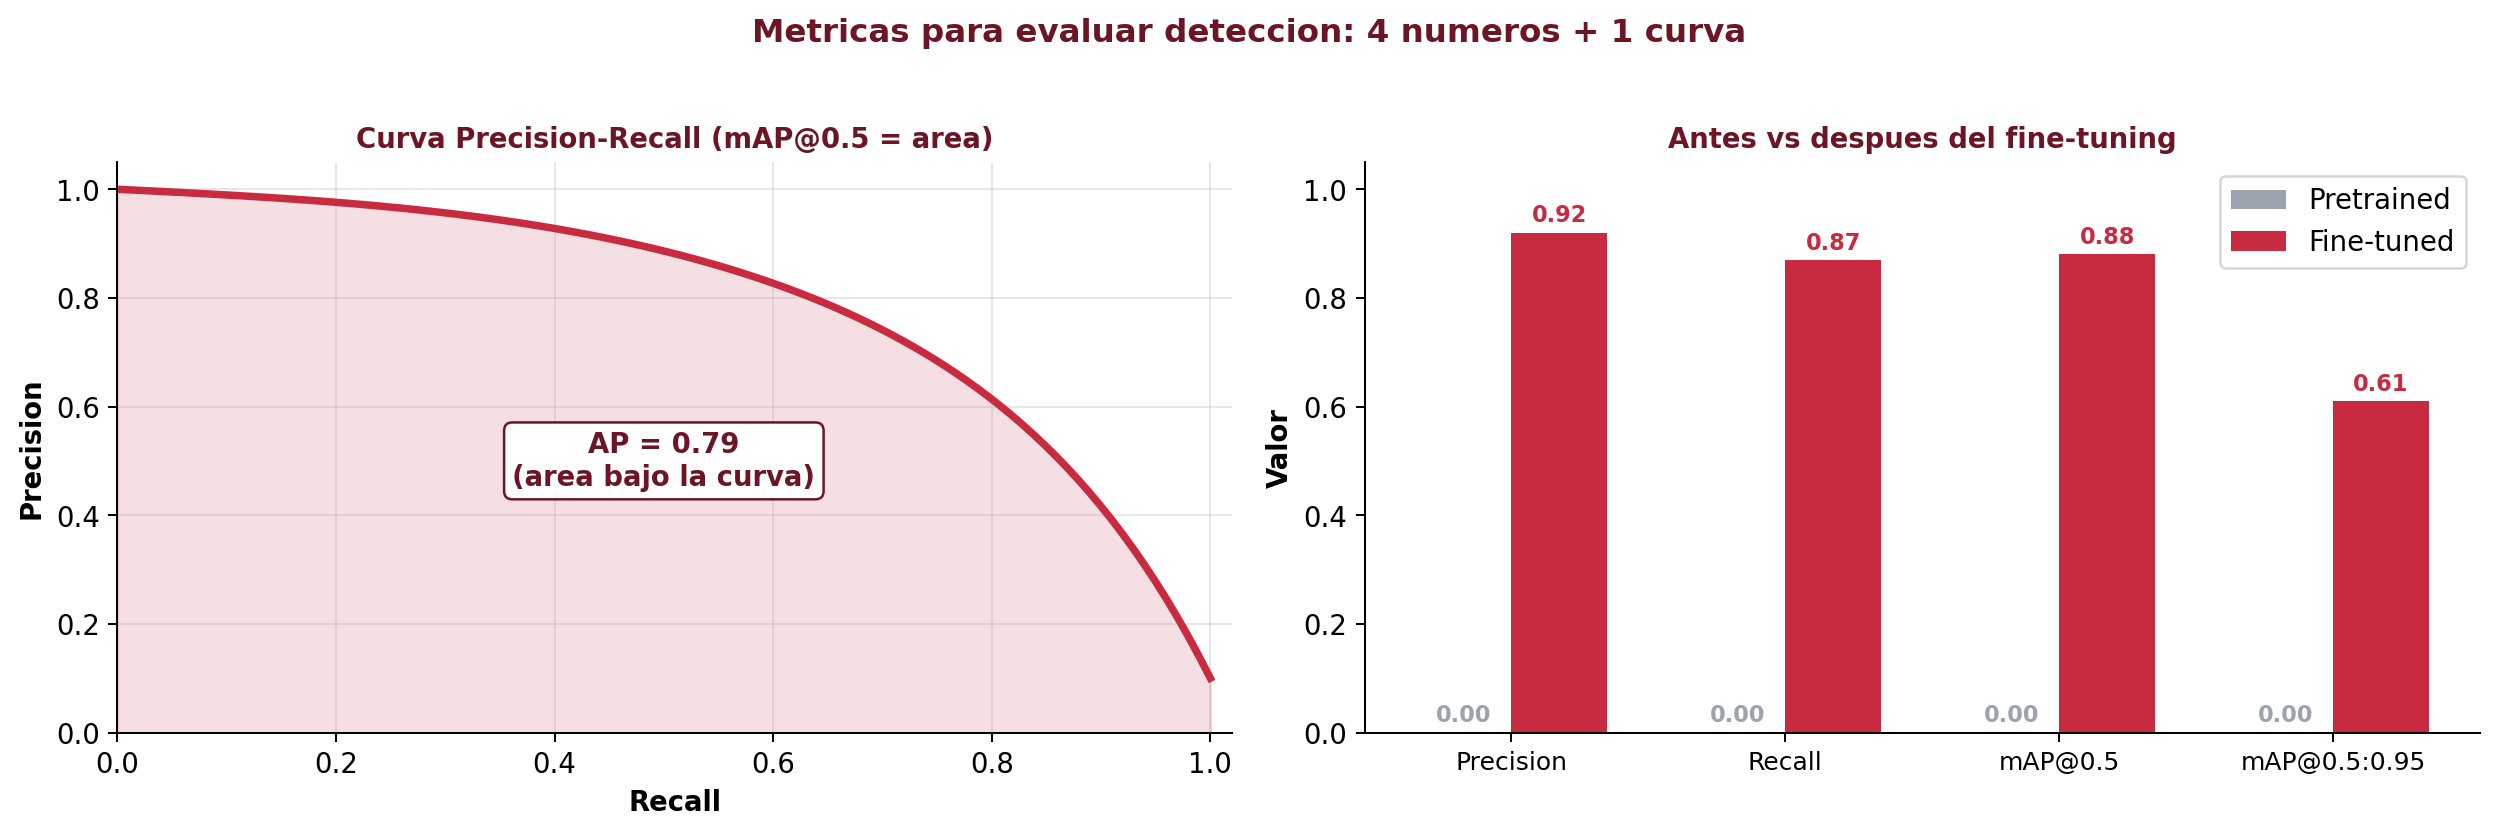
\includegraphics[width=0.97\textwidth]{fig_metrics.png}
  \end{center}

  \vspace{4pt}
  {\scriptsize\color{textMuted}
    \faLightbulb\hspace{4pt} \textbf{Izquierda:} curva P-R --- el \'area bajo
    la curva es el AP. \textbf{Derecha:} pretrained YOLO no detecta placas
    (0\%); fine-tuned salta a 88\%.}
\end{frame}

\begin{frame}[shrink]{Trade-offs Pr\'acticos}
  \vspace{8pt}
  {\footnotesize
  \begin{tabular}{@{}p{3.5cm} p{3.5cm} p{5.0cm}@{}}
    \toprule
    \textbf{Bot\'on que mueves} & \textbf{Sube} & \textbf{Baja} \\
    \midrule
    \rowcolor{arcaGray}
    \texttt{conf\_threshold} alto
    & Precision
    & Recall (te pierdes objetos) \\
    \texttt{conf\_threshold} bajo
    & Recall
    & Precision (m\'as falsos positivos) \\
    \rowcolor{arcaGray}
    Imagen 640px $\to$ 1280px
    & Recall (objetos peque\~nos)
    & Velocidad \\
    Modelo nano $\to$ medium
    & Precision general
    & Velocidad y memoria \\
    \bottomrule
  \end{tabular}
  }

  \vspace{14pt}
  \begin{tcolorbox}[colback=arcaGray, colframe=arcaRed, boxrule=0.5pt,
    arc=2pt, left=6pt, right=6pt, top=4pt, bottom=4pt]
    {\scriptsize\color{arcaDark}
    \faExclamationTriangle\hspace{4pt} La m\'etrica importante depende del caso.
    Cl\'inica prioriza \textbf{recall} (no perder un tumor).
    Control de acceso prioriza \textbf{precision} (no abrir a un auto equivocado).}
  \end{tcolorbox}
\end{frame}

% =============================================================================
%  FINE-TUNING DESDE LA NECESIDAD
% =============================================================================
\sectionframe{Fine-Tuning Desde la Necesidad}{COCO no tiene lo que necesitamos}

\begin{frame}[shrink]{Las 80 Clases de COCO}
  \vspace{4pt}
  \begin{center}
    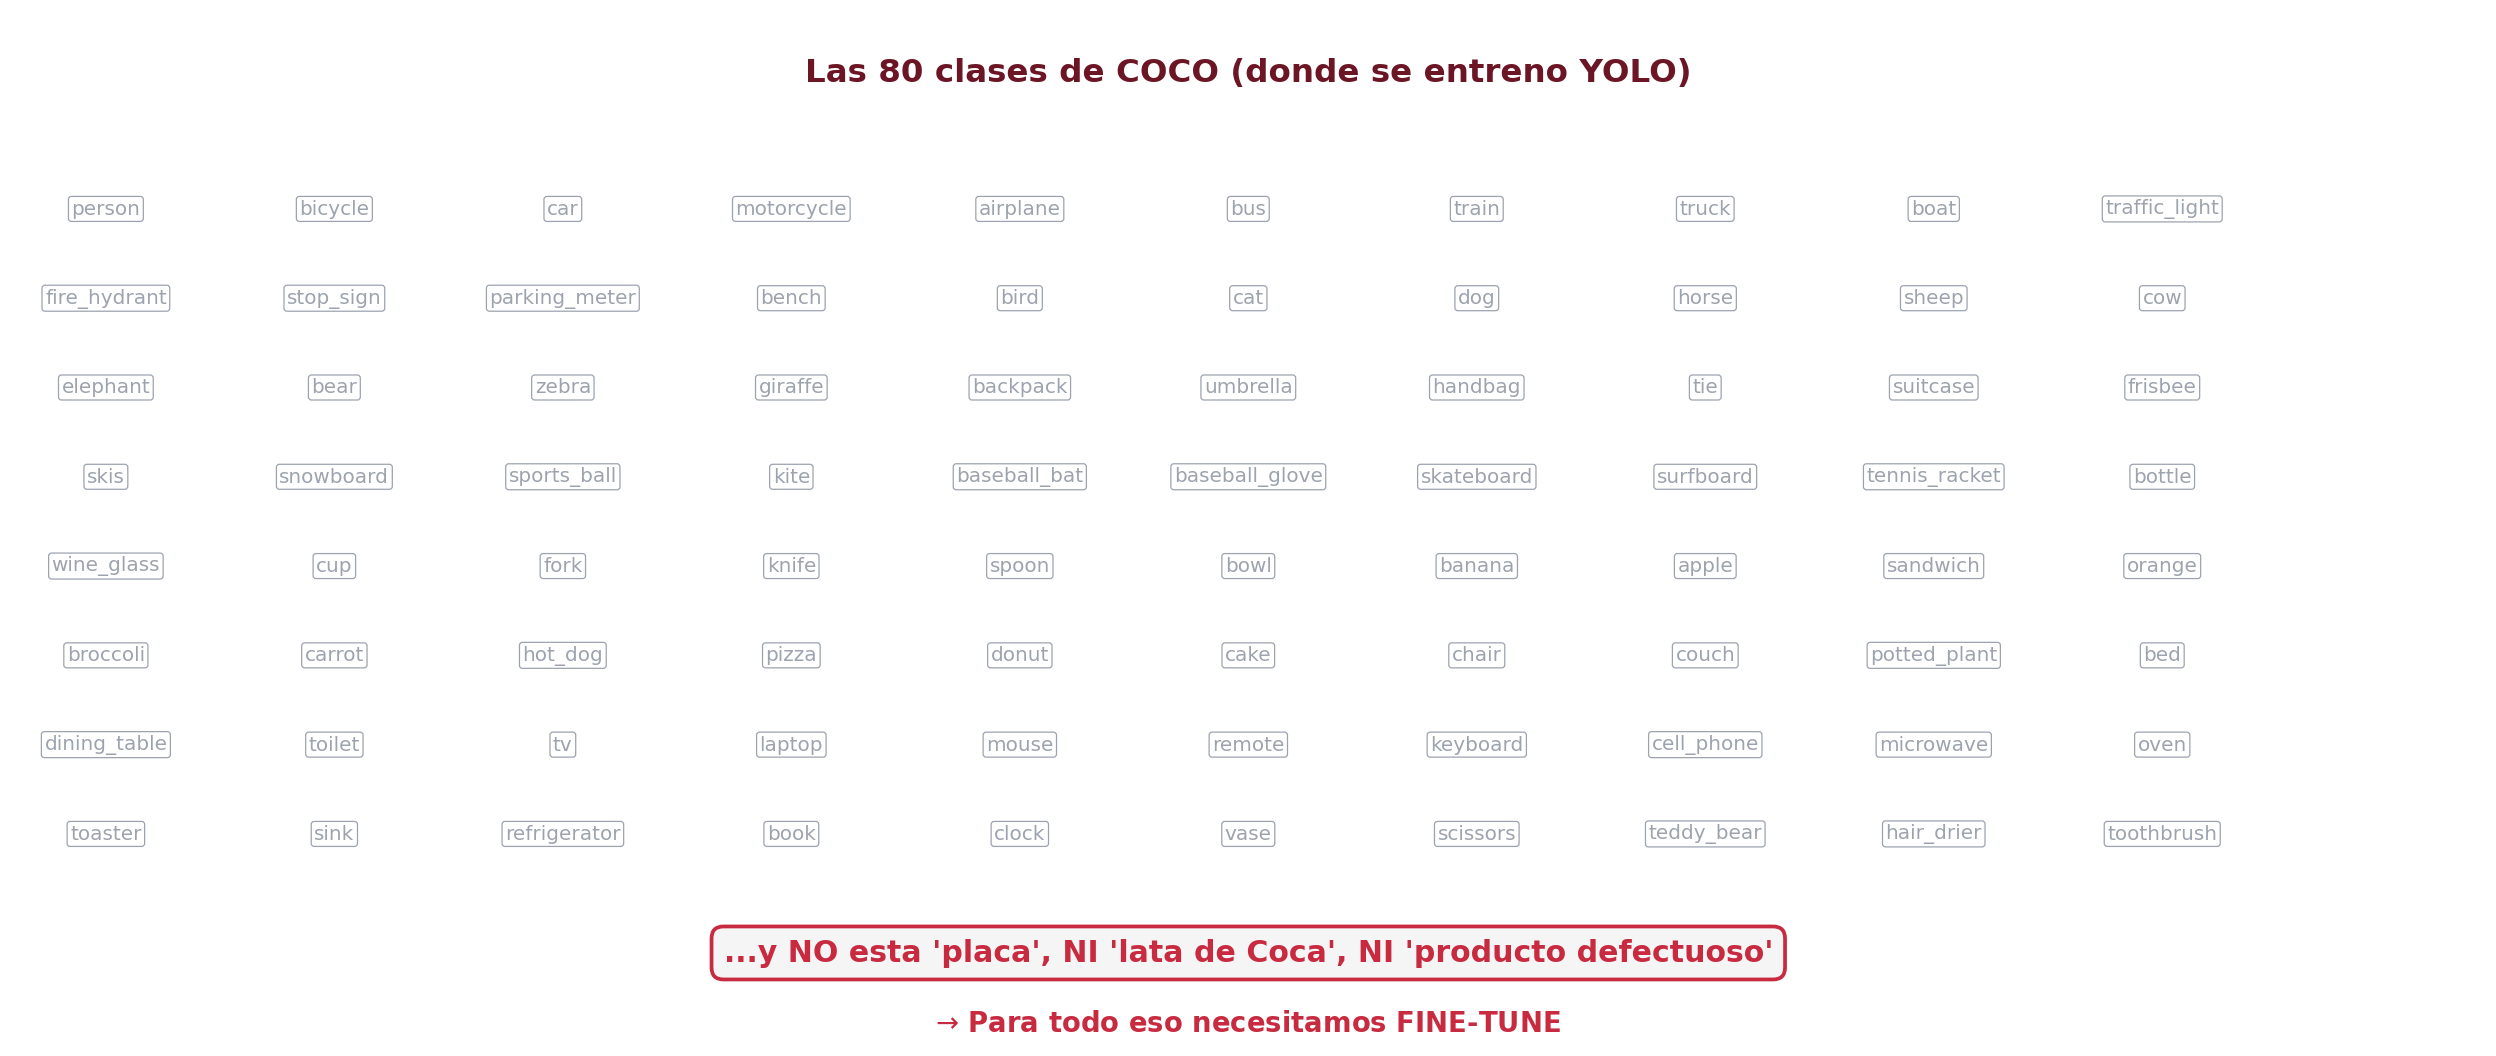
\includegraphics[width=0.97\textwidth]{fig_coco_classes.png}
  \end{center}

  \vspace{2pt}
  {\scriptsize\color{textMuted}
    \faLightbulb\hspace{4pt} COCO tiene autos, perros, sillas, sand\'wiches.
    Pero \textbf{no tiene placa, ni lata-de-Coca, ni producto-defectuoso}.
    Casi todos los problemas industriales reales requieren clases que
    COCO no incluye.}
\end{frame}

\begin{frame}[shrink]{El Pretrained NO Detecta Lo Que Te Importa}
  \vspace{8pt}
  {\footnotesize\color{arcaDark}\bfseries
    Si en la clase 25 corrimos YOLO26 pretrained sobre una foto de carro,
    detect\'o \texttt{car}, quiz\'a \texttt{truck}.
    \textbf{Pero NUNCA detect\'o \texttt{license\_plate}.} Porque no existe esa clase.}

  \vspace{14pt}
  {\footnotesize
  \begin{itemize}\setlength{\itemsep}{6pt}
    \item[{\color{arcaRed}\scriptsize\faTimes}]
      Pretrained YOLO26 sobre placas: \textbf{mAP@0.5 = 0\%}
    \item[{\color{arcaRed}\scriptsize\faTimes}]
      Esto NO es un bug del modelo. Es que COCO nunca tuvo esa clase.
    \item[{\color{codeGreen}\scriptsize\faArrowRight}]
      \textbf{Soluci\'on:} fine-tune. Reentrenar el cabezal con \emph{nuestros}
      datos etiquetados para que aprenda la clase \texttt{placa}.
    \item[{\color{codeGreen}\scriptsize\faArrowRight}]
      \textbf{La misma idea} de la clase 24: backbone congelado + cabezal nuevo.
  \end{itemize}
  }
\end{frame}

\begin{frame}[shrink]{Fine-Tuning Es Lo Mismo Que Vimos}
  \vspace{4pt}
  \begin{center}
    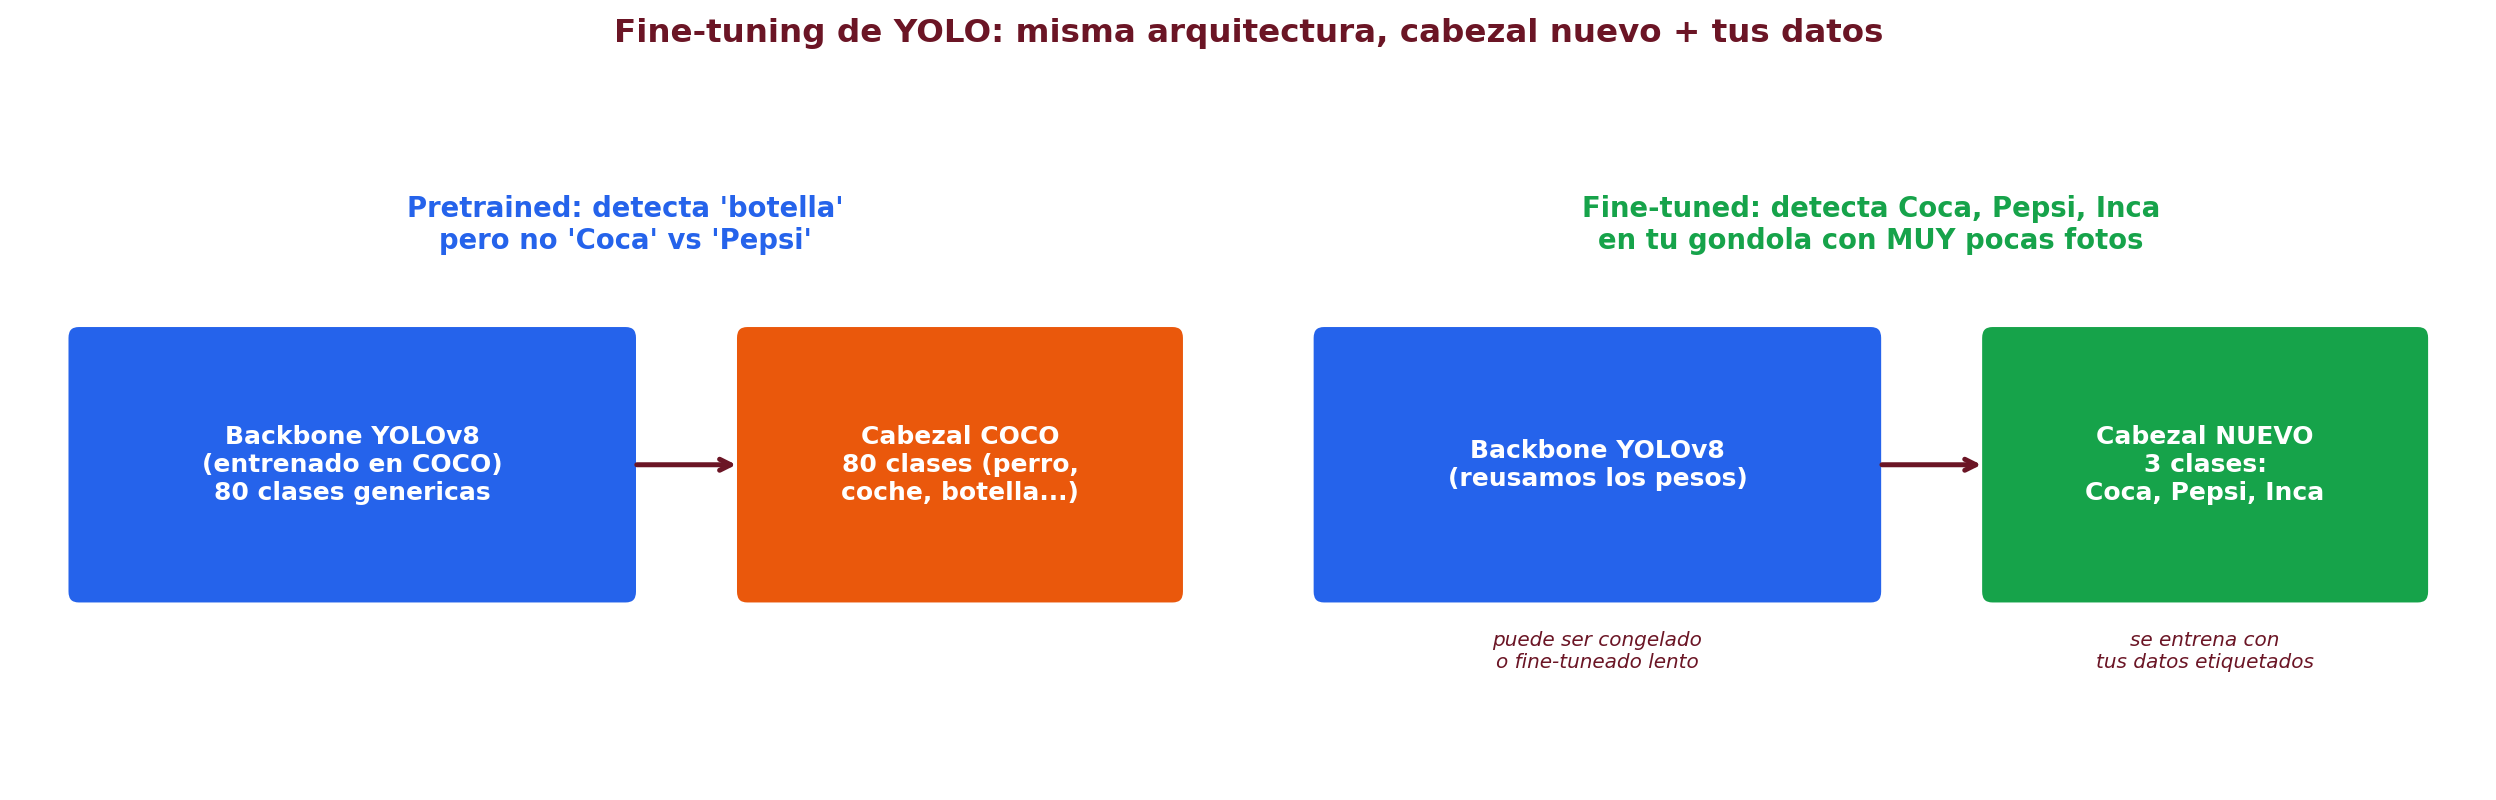
\includegraphics[width=0.85\textwidth]{fig_finetune.png}
  \end{center}

  \vspace{4pt}
  {\scriptsize\color{textMuted}
    \faLightbulb\hspace{4pt} \textbf{En clase 24 (clasificaci\'on)}: VGG16
    preentrenado + cabezal Dense nuevo. \textbf{Hoy (detecci\'on)}: YOLO26
    preentrenado + cabezal de detecci\'on para \texttt{placa}.
    Cambia el tipo de cabeza, no la idea.}
\end{frame}

\begin{frame}[shrink]{Qu\'e Necesitamos Para Fine-Tunear}
  \vspace{8pt}
  {\footnotesize
  \begin{tabular}{@{}p{2.5cm} p{4.5cm} p{5.0cm}@{}}
    \toprule
    \textbf{Ingrediente} & \textbf{Qu\'e es} & \textbf{D\'onde lo conseguimos} \\
    \midrule
    \rowcolor{arcaGray}
    Im\'agenes
    & Fotos de carros con placas visibles
    & ZIP en el repo (100 imgs sin labels) \\
    Etiquetas
    & Bbox dibujado por humanos
    & \textbf{Nosotros lo hacemos hoy en equipo} \\
    \rowcolor{arcaGray}
    Modelo base
    & YOLO26n pretrained en COCO
    & Ultralytics lo baja autom\'aticamente \\
    GPU
    & Para entrenar en pocos minutos
    & Colab T4 gratis \\
    \rowcolor{arcaGray}
    Tiempo
    & 10--15 min de fine-tune
    & Lo corremos en vivo en clase \\
    \bottomrule
  \end{tabular}
  }
\end{frame}

% =============================================================================
%  EQUIPO DE ANNOTATION CON LABEL STUDIO
% =============================================================================
\sectionframe{Somos un Equipo de Annotation}{Como en cualquier empresa de IA seria}

\begin{frame}[shrink]{La Realidad: Datos Sin Etiquetar No Sirven}
  \vspace{8pt}
  {\footnotesize\color{arcaDark}\bfseries
    En toda empresa de IA seria hay un \textbf{equipo dedicado solo a etiquetar}.
    Es la actividad m\'as costosa del ciclo --- y la m\'as cr\'itica para la
    calidad del modelo.}

  \vspace{14pt}
  {\footnotesize
  \begin{itemize}\setlength{\itemsep}{6pt}
    \item[{\color{arcaRed}\scriptsize\faArrowRight}]
      Empresas como Scale AI, Surge AI, Appen viven de hacer este trabajo
      (vendieron por \$miles de millones).
    \item[{\color{arcaRed}\scriptsize\faArrowRight}]
      Tesla, Waymo, OpenAI tienen \textbf{cientos} de etiquetadores internos.
    \item[{\color{codeGreen}\scriptsize\faArrowRight}]
      Hoy nosotros somos ese equipo. Roles, herramientas y workflow profesionales.
  \end{itemize}
  }
\end{frame}

\begin{frame}[shrink]{Roles del Equipo}
  \vspace{4pt}
  \begin{center}
    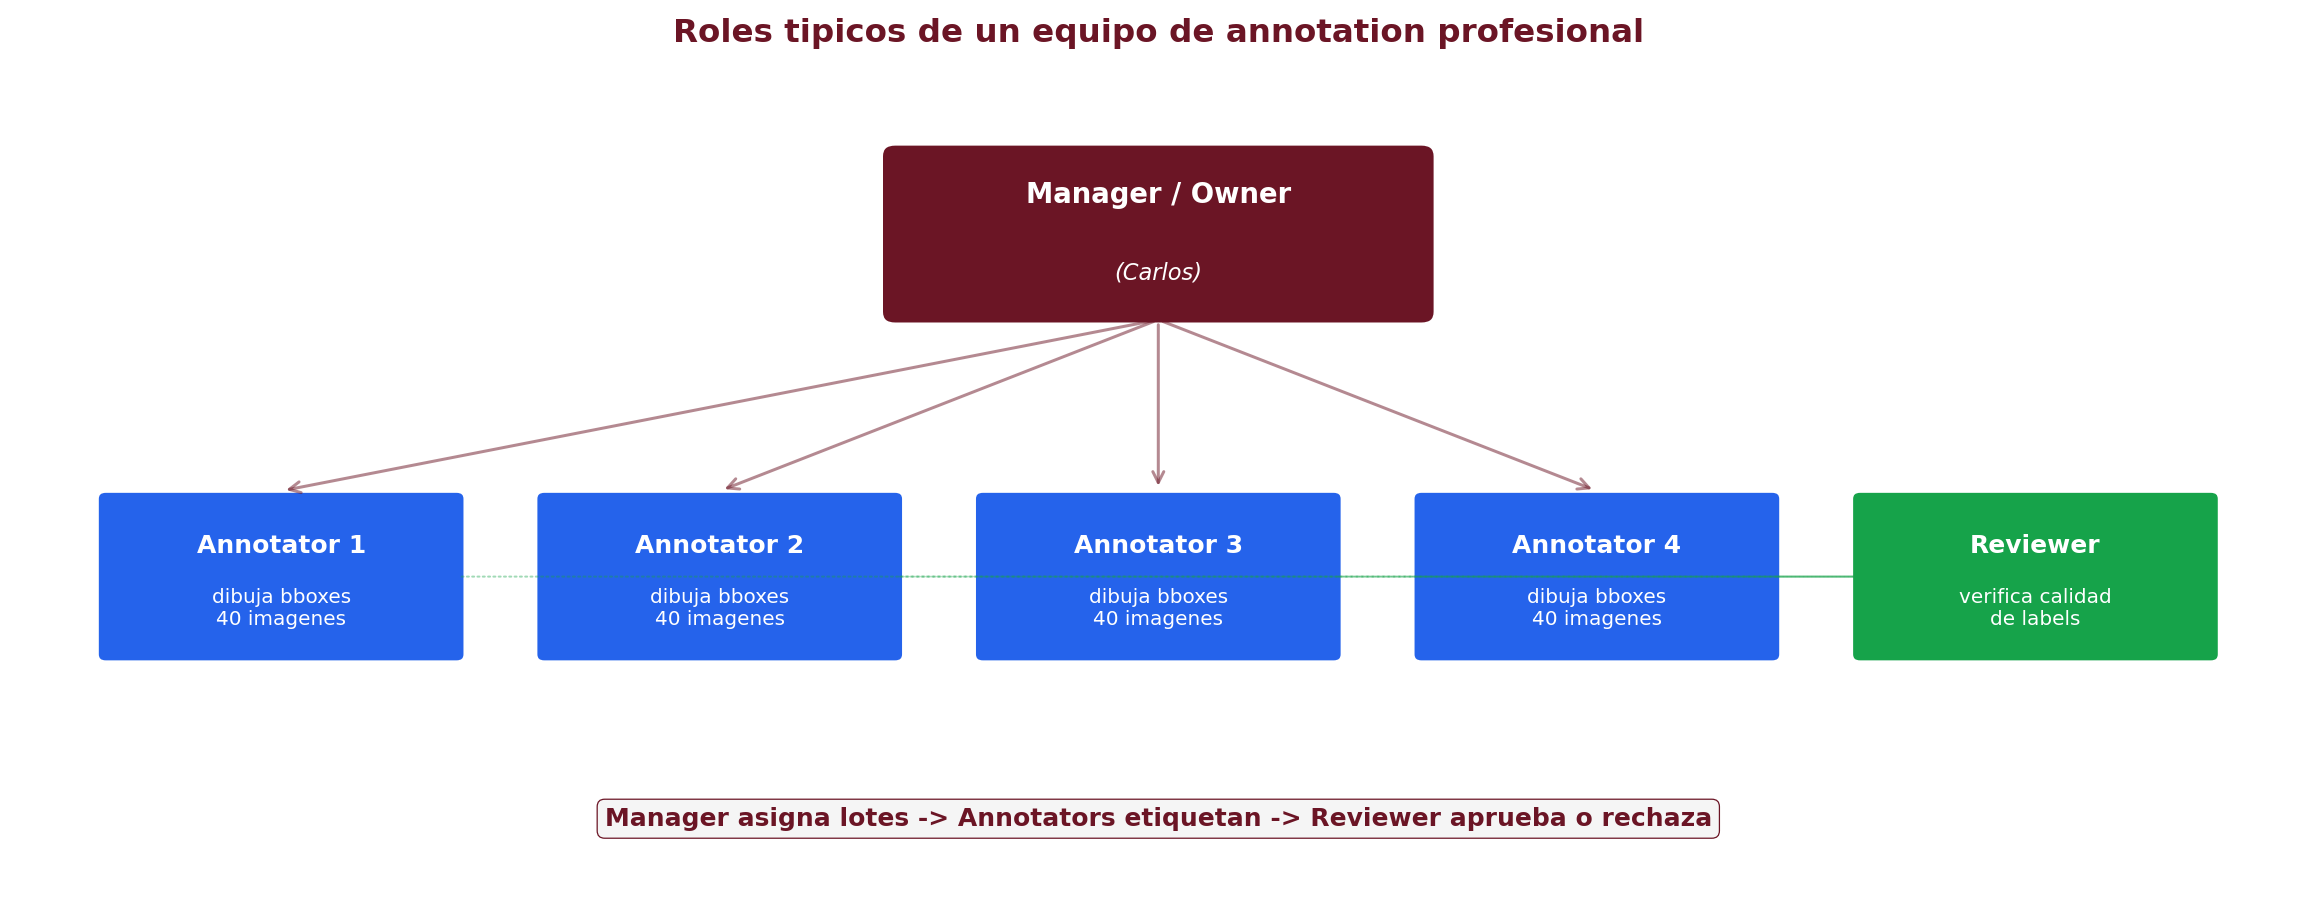
\includegraphics[width=0.97\textwidth]{fig_team_roles.png}
  \end{center}

  \vspace{2pt}
  {\scriptsize\color{textMuted}
    \faLightbulb\hspace{4pt} \textbf{Manager} asigna lotes y aprueba.
    \textbf{Annotators} (la mayor\'ia) dibujan bboxes.
    \textbf{Reviewer} (1--2 voluntarios) revisa calidad antes de aceptar.}
\end{frame}

\begin{frame}[shrink]{Herramienta: Label Studio (hospedado en Railway)}
  \vspace{4pt}
  \begin{center}
    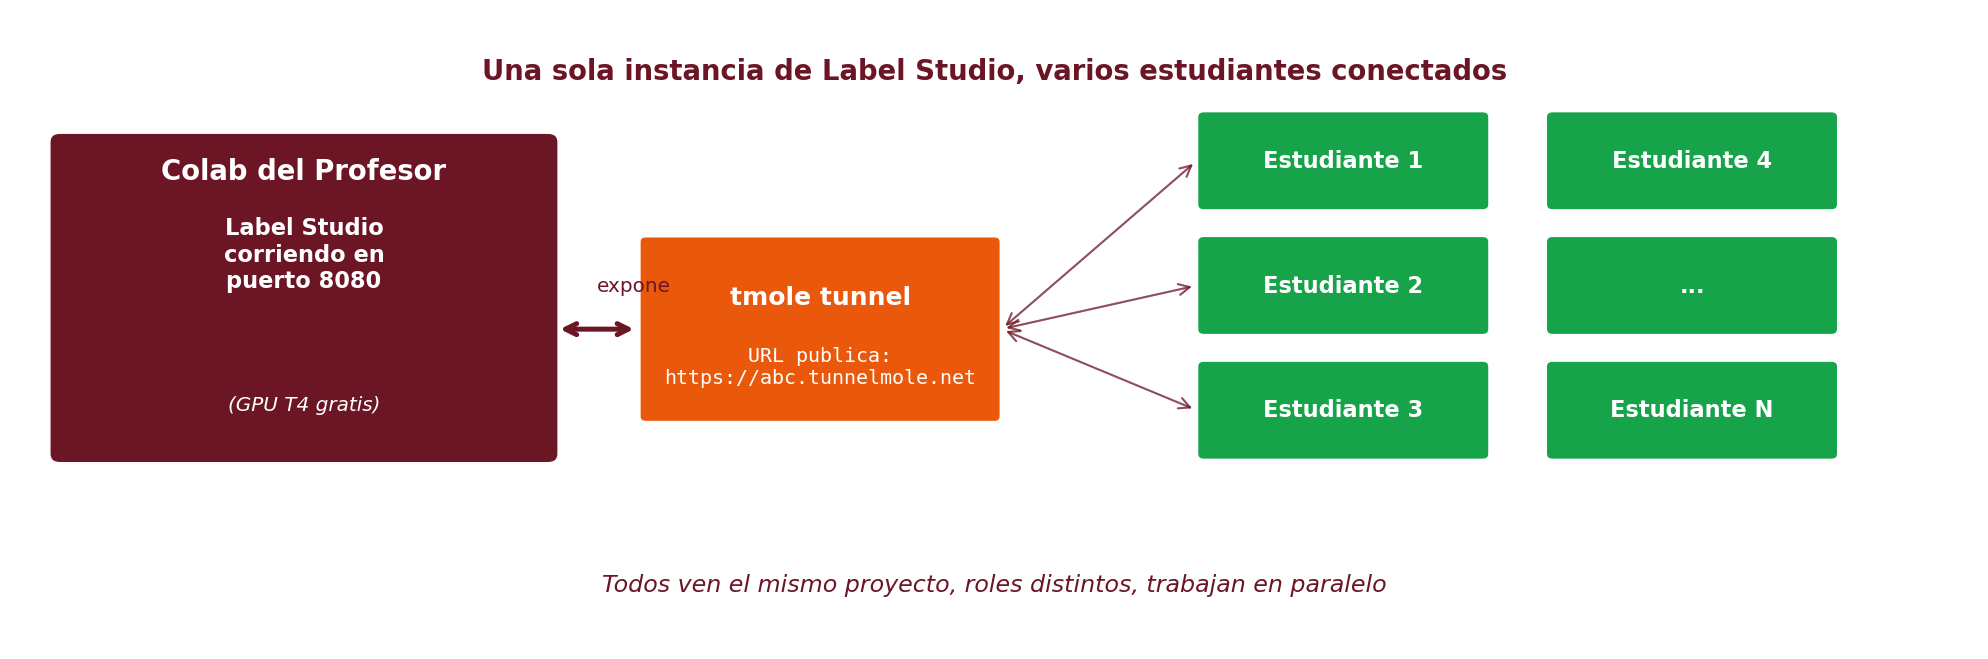
\includegraphics[width=0.95\textwidth]{fig_labelstudio_setup.png}
  \end{center}

  \vspace{8pt}
  \begin{tcolorbox}[colback=arcaGray, colframe=arcaRed, boxrule=0.5pt,
    arc=2pt, left=6pt, right=6pt, top=4pt, bottom=4pt]
    {\scriptsize\color{arcaDark}
    \faGlobe\hspace{4pt}\textbf{URL del servidor de la clase:}\\[2pt]
    \texttt{\small https://label-studio-production-281f.up.railway.app/}}
  \end{tcolorbox}

  \vspace{6pt}
  {\scriptsize\color{textMuted}
    \faLightbulb\hspace{4pt} Label Studio corriendo en Railway (gratis,
    persistente entre clases). Cada estudiante crea cuenta en esa URL,
    el profesor le asigna lotes, todos trabajan en paralelo sobre el
    mismo proyecto.}
\end{frame}

\begin{frame}[shrink]{Conectar el Dataset Etiquetado a Python}
  \vspace{6pt}
  {\footnotesize\color{arcaDark}\bfseries
    Label Studio expone una \textbf{REST API}. Desde el notebook de
    training bajamos los labels directo --- sin click manual en Export.}

  \vspace{12pt}
  {\footnotesize
  \begin{itemize}\setlength{\itemsep}{6pt}
    \item[{\color{arcaRed}\scriptsize\faArrowRight}]
      Endpoint: \texttt{GET /api/projects/\{id\}/export?exportType=YOLO}
    \item[{\color{arcaRed}\scriptsize\faArrowRight}]
      Autenticaci\'on: \texttt{Authorization: Bearer <access\_token>}
    \item[{\color{arcaRed}\scriptsize\faArrowRight}]
      Si el token es JWT \texttt{refresh}, primero intercambiar por
      \texttt{access} en \texttt{/api/token/refresh/}.
    \item[{\color{codeGreen}\scriptsize\faArrowRight}]
      Responde un ZIP con \texttt{labels/*.txt} en formato YOLO.
      Lo emparejamos con las im\'agenes locales por nombre de archivo.
  \end{itemize}
  }
\end{frame}

\begin{frame}[fragile,shrink]{C\'odigo: Bajar el Dataset desde Python}
  \vspace{-4pt}
  \begin{pyblock}
import requests, zipfile, io

BASE_URL = "https://label-studio-production-281f.up.railway.app"
REFRESH_TOKEN = "eyJhbGc..."     # token JWT de tu cuenta

# 1. Intercambiar refresh por access token
r = requests.post(f"{BASE_URL}/api/token/refresh/",
                  json={"refresh": REFRESH_TOKEN})
access = r.json()["access"]
headers = {"Authorization": f"Bearer {access}"}

# 2. Bajar export YOLO del proyecto
r = requests.get(f"{BASE_URL}/api/projects/1/export",
                 params={"exportType": "YOLO"}, headers=headers)

# 3. Extraer el ZIP de labels
zipfile.ZipFile(io.BytesIO(r.content)).extractall("ls_export")
  \end{pyblock}
\end{frame}

\begin{frame}[shrink]{Workflow del Equipo Hoy}
  \vspace{8pt}
  {\footnotesize
  \begin{enumerate}\setlength{\itemsep}{6pt}
    \item[{\color{arcaRed}\bfseries 1.}]
      Abrir
      \texttt{\scriptsize https://label-studio-production-281f.up.railway.app/}
    \item[{\color{arcaRed}\bfseries 2.}]
      Cada estudiante crea cuenta y se loguea.
    \item[{\color{arcaRed}\bfseries 3.}]
      Proyecto ya creado: ``Placas'' (label \'unica \texttt{placa},
      100 im\'agenes precargadas).
    \item[{\color{arcaRed}\bfseries 4.}]
      Asignaci\'on de lotes: cada estudiante etiqueta $\sim$5--10
      im\'agenes (15--20 min).
    \item[{\color{arcaRed}\bfseries 5.}]
      Reviewers verifican y aceptan o piden correcci\'on.
    \item[{\color{codeGreen}\bfseries 6.}]
      El notebook de training baja los labels v\'ia REST API y los
      empareja con las im\'agenes locales.
  \end{enumerate}
  }
\end{frame}

\begin{frame}[shrink]{Buenas Pr\'acticas Profesionales}
  \vspace{8pt}
  {\footnotesize
  \begin{itemize}\setlength{\itemsep}{6pt}
    \item[{\color{arcaRed}\scriptsize\faArrowRight}]
      \textbf{Guidelines escritas}: ``placa = el rect\'angulo de la placa,
      ajustado, sin margen''.
    \item[{\color{arcaRed}\scriptsize\faArrowRight}]
      \textbf{Inter-annotator agreement (IAA)}: 2 personas etiquetan la
      misma imagen, medir cu\'anto coinciden. Bajo IAA = guidelines ambiguas.
    \item[{\color{arcaRed}\scriptsize\faArrowRight}]
      \textbf{Pilot batch}: etiquetar 20 im\'agenes primero, revisar,
      ajustar guidelines, luego masivo.
    \item[{\color{arcaRed}\scriptsize\faArrowRight}]
      \textbf{Casos l\'imite documentados}: placas borrosas, parciales,
      truncadas $\to$ regla expl\'icita.
    \item[{\color{codeGreen}\scriptsize\faArrowRight}]
      \textbf{Backup peri\'odico}: exportar cada hora por si Colab se cae.
  \end{itemize}
  }
\end{frame}

% =============================================================================
%  FINE-TUNE EN VIVO
% =============================================================================
\sectionframe{Fine-Tune en Vivo}{Mientras explico, el modelo aprende}

\begin{frame}[fragile,shrink]{Estructura del Dataset Para YOLO}
  \vspace{-4pt}
  \begin{pyblock}
# Despues de exportar de Label Studio en formato YOLO,
# Consolidar en este layout:
#
# dataset/
#   |-- images/
#   |    |-- train/      <- 80 imagenes
#   |    `-- val/        <- 20 imagenes
#   |-- labels/
#   |    |-- train/      <- 1 .txt por imagen
#   |    `-- val/
#   `-- data.yaml        <- paths + clases

# Contenido de data.yaml:
yaml_text = '''
path: /content/dataset
train: images/train
val:   images/val

names:
  0: placa
'''
  \end{pyblock}
\end{frame}

\begin{frame}[fragile,shrink]{Fine-Tune en 5 L\'ineas}
  \vspace{-4pt}
  \begin{pyblock}
from ultralytics import YOLO

# 1. Cargar pretrained
model = YOLO("yolo26n.pt")

# 2. Fine-tune (corre en GPU T4 de Colab gratis)
results = model.train(
    data="dataset/data.yaml",
    epochs=30,
    imgsz=640,
    batch=16,
    patience=5,   # early stopping si val no mejora en 5 epochs
)

# 3. Evaluar
metrics = model.val()
print(f"mAP@0.5      = {metrics.box.map50:.3f}")
print(f"mAP@0.5:0.95 = {metrics.box.map:.3f}")
print(f"Precision    = {metrics.box.mp:.3f}")
print(f"Recall       = {metrics.box.mr:.3f}")
  \end{pyblock}
\end{frame}

\begin{frame}[shrink]{Mientras Entrena, Qu\'e Mirar}
  \vspace{8pt}
  {\footnotesize
  \begin{itemize}\setlength{\itemsep}{6pt}
    \item[{\color{arcaRed}\scriptsize\faArrowRight}]
      \textbf{box\_loss}: error de las coordenadas (x, y, w, h). Debe bajar.
    \item[{\color{arcaRed}\scriptsize\faArrowRight}]
      \textbf{cls\_loss}: error de clasificaci\'on. Debe bajar.
    \item[{\color{arcaRed}\scriptsize\faArrowRight}]
      \textbf{val\_loss}: si sube mientras train\_loss baja $\to$ overfitting.
    \item[{\color{arcaRed}\scriptsize\faArrowRight}]
      \textbf{mAP@0.5}: debe ir subiendo cada epoch. Si se estanca $\to$
      learning rate muy alto/bajo, o dataset chico.
    \item[{\color{codeGreen}\scriptsize\faArrowRight}]
      \textbf{best.pt}: Ultralytics guarda autom\'aticamente el checkpoint
      con el mejor mAP. Usarlo, no el \'ultimo.
  \end{itemize}
  }
\end{frame}

\begin{frame}[shrink]{Antes / Despu\'es del Fine-Tune}
  \vspace{4pt}
  \begin{center}
    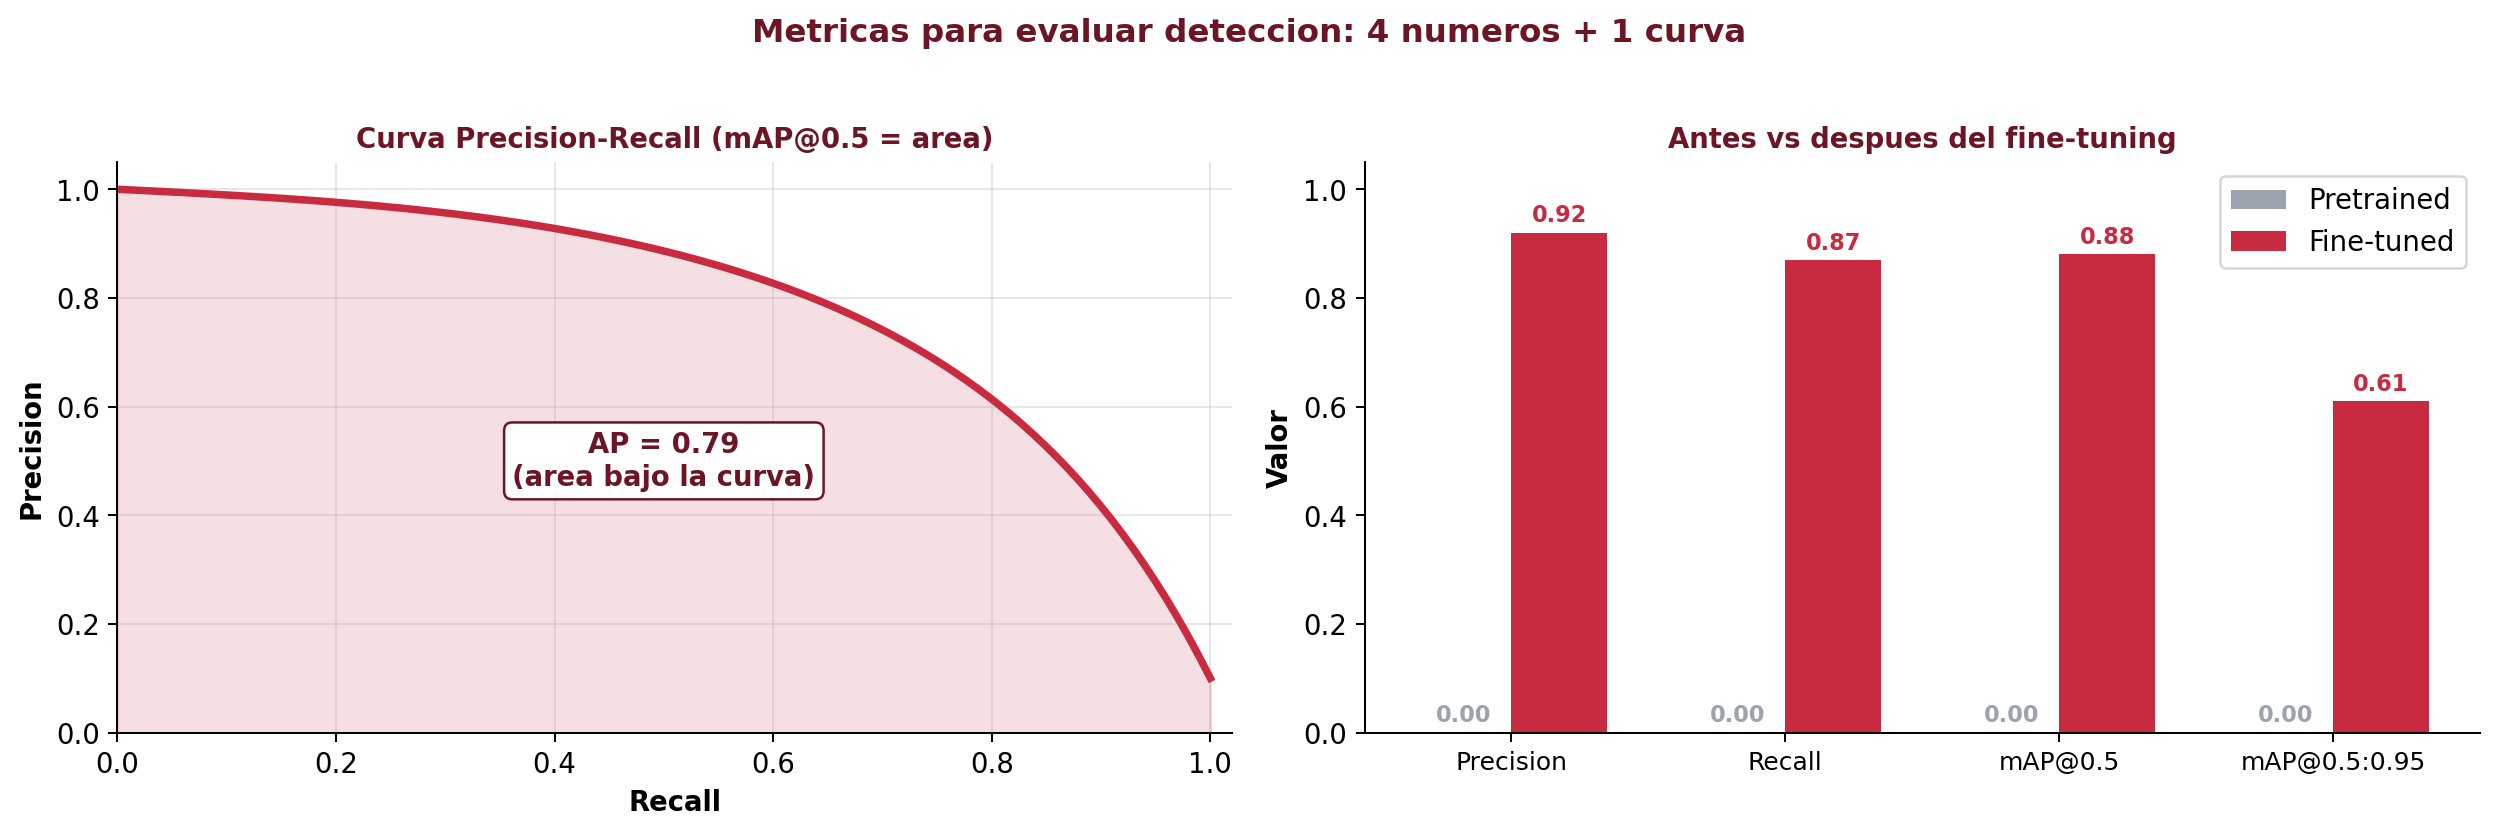
\includegraphics[width=0.97\textwidth]{fig_metrics.png}
  \end{center}

  \vspace{4pt}
  {\scriptsize\color{textMuted}
    \faLightbulb\hspace{4pt} \textbf{Antes}: pretrained sobre placas $=$ 0\%.
    \textbf{Despu\'es}: $\sim$88\% mAP@0.5 con apenas $\sim$300 im\'agenes
    etiquetadas en equipo. Eso es el poder de fine-tuning bien hecho.}
\end{frame}

% =============================================================================
%  OCR CASCADE + GRADIO
% =============================================================================
\sectionframe{OCR Cascade + App}{Detectar + leer + desplegar}

\begin{frame}[shrink]{El Pipeline Completo}
  \vspace{4pt}
  \begin{center}
    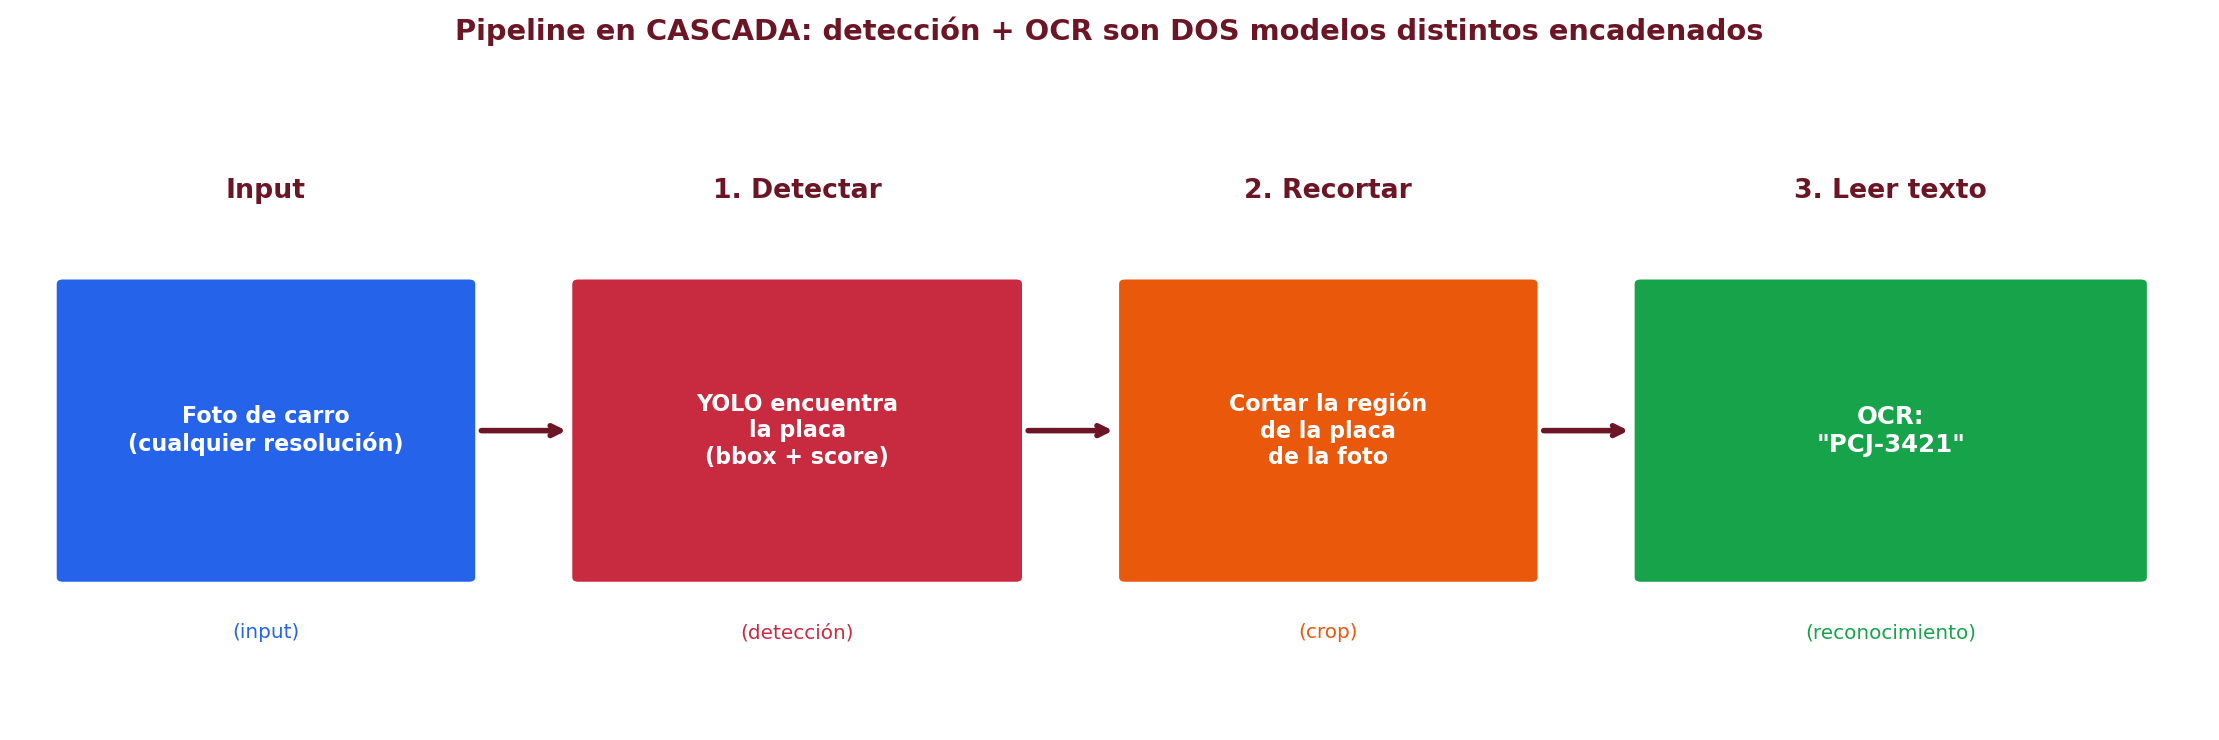
\includegraphics[width=0.95\textwidth]{fig_ocr_cascade_diagram.png}
  \end{center}

  \vspace{4pt}
  {\scriptsize\color{textMuted}
    \faLightbulb\hspace{4pt} \textbf{Dos modelos encadenados}:
    YOLO fine-tuneado encuentra la placa, EasyOCR lee el texto.
    Cada uno hace una sola cosa muy bien.}
\end{frame}

\begin{frame}[shrink]{?`Qu\'e Es EasyOCR?}
  \vspace{6pt}
  {\footnotesize\color{arcaDark}\bfseries
    Librer\'ia Python open source (JaidedAI) para leer texto en
    im\'agenes. Soporta \textbf{80+ idiomas} (incluido espa\~nol).
    Una sola l\'inea para arrancar.}

  \vspace{14pt}
  {\footnotesize
  \begin{itemize}\setlength{\itemsep}{6pt}
    \item[{\color{arcaRed}\scriptsize\faArrowRight}]
      \texttt{pip install easyocr} y listo. Baja los modelos
      autom\'aticamente la primera vez.
    \item[{\color{arcaRed}\scriptsize\faArrowRight}]
      Funciona con \texttt{numpy arrays}, archivos JPG/PNG o URLs.
    \item[{\color{arcaRed}\scriptsize\faArrowRight}]
      Devuelve la lista de \texttt{(bbox, texto, confianza)} para cada
      pedazo de texto encontrado.
    \item[{\color{codeGreen}\scriptsize\faArrowRight}]
      Compite con Tesseract (m\'as viejo) y PaddleOCR (m\'as preciso
      pero pesado). EasyOCR es el \textbf{balance pr\'actico}.
  \end{itemize}
  }
\end{frame}

\begin{frame}[shrink]{Por Dentro: Pipeline de 2 Etapas}
  \vspace{6pt}
  {\footnotesize\color{arcaDark}\bfseries
    EasyOCR \emph{no} es un modelo. Son \textbf{dos redes neuronales
    encadenadas}, parecido a lo que hicimos hoy con YOLO + OCR pero a
    otra escala.}

  \vspace{14pt}
  {\footnotesize
  \begin{enumerate}\setlength{\itemsep}{8pt}
    \item[{\color{arcaRed}\bfseries 1.}]
      \textbf{Detecci\'on de texto --- CRAFT} (Character Region Awareness for
      Text Detection). Una CNN tipo VGG/UNet que predice dos heatmaps:
      \emph{centros de car\'acter} y \emph{enlaces entre caracteres}.
      Sale una lista de pol\'igonos donde hay texto.
    \item[{\color{arcaRed}\bfseries 2.}]
      \textbf{Reconocimiento --- CRNN} (Convolutional Recurrent Neural Network).
      Para cada pol\'igono: \textbf{CNN} extrae features visuales,
      \textbf{BiLSTM} modela la secuencia de caracteres,
      \textbf{CTC decoder} alinea features con caracteres de longitud variable.
    \item[{\color{codeGreen}\bfseries 3.}]
      Opcional: modelo de lenguaje (n-grams) para corregir errores
      en texto natural. \textbf{Para placas se desactiva}
      (\texttt{paragraph=False}) porque son aleatorias, no palabras.
  \end{enumerate}
  }
\end{frame}

\begin{frame}[shrink]{?`C\'omo La Pueden Usar en Sus Proyectos?}
  \vspace{6pt}
  {\footnotesize
  \begin{tabular}{@{}p{4.5cm} p{8.0cm}@{}}
    \toprule
    \textbf{Caso de uso} & \textbf{Patr\'on} \\
    \midrule
    \rowcolor{arcaGray}
    Leer factura / recibo
    & EasyOCR sobre la foto completa, \texttt{paragraph=True} \\
    Leer placa de cami\'on al entrar a planta
    & YOLO detecta placa $\to$ recorta $\to$ EasyOCR sobre el recorte \\
    \rowcolor{arcaGray}
    Leer fecha de vencimiento en empaque
    & YOLO detecta zona de impresi\'on $\to$ EasyOCR sobre el recorte \\
    Digitalizar documentos en bodega
    & EasyOCR pagina completa, luego post-proceso con regex \\
    \rowcolor{arcaGray}
    Leer n\'umero de serie en pieza
    & Recortar manualmente $\to$ EasyOCR + filtros de regex \\
    \bottomrule
  \end{tabular}
  }

  \vspace{10pt}
  \begin{tcolorbox}[colback=codeGreen!8, colframe=codeGreen, boxrule=0.5pt,
    arc=2pt, left=6pt, right=6pt, top=4pt, bottom=4pt]
    {\scriptsize\color{arcaDark}
    \faKey\hspace{4pt}\textbf{Tip industrial:} \emph{recortar antes de
    leer} mejora muchisimo. EasyOCR sobre la foto completa es lento y se
    confunde con texto irrelevante. Por eso encadenamos detecci\'on + OCR.}
  \end{tcolorbox}
\end{frame}

\begin{frame}[shrink]{Limitaciones y Alternativas}
  \vspace{6pt}
  {\footnotesize
  \begin{tabular}{@{}p{3.5cm} p{8.7cm}@{}}
    \toprule
    \textbf{Limitaci\'on} & \textbf{Soluci\'on} \\
    \midrule
    \rowcolor{arcaGray}
    Texto muy rotado / vertical
    & EasyOCR soporta rotaci\'on hasta $\sim$45$^\circ$. M\'as que eso,
      hay que rotar antes con OpenCV. \\
    Letras manuscritas
    & Falla. Usar \textbf{TrOCR} (Microsoft, transformer) para handwriting. \\
    \rowcolor{arcaGray}
    Texto industrial muy peque\~no
    & Sube la resoluci\'on del crop (resize 2--3$\times$) antes de leer. \\
    Velocidad cr\'itica
    & \textbf{PaddleOCR} es 3--5$\times$ m\'as r\'apido en CPU. \\
    \rowcolor{arcaGray}
    Idiomas no latinos
    & EasyOCR los maneja (chino, \'arabe, japon\'es, hindi). \\
    M\'axima precisi\'on en placas
    & Entrenar un \textbf{CRNN espec\'ifico} de placas en vez de OCR
      gen\'erico. \\
    \bottomrule
  \end{tabular}
  }

  \vspace{8pt}
  {\scriptsize\color{textMuted}
    \faLightbulb\hspace{4pt} EasyOCR es el \textbf{default razonable} para
    cualquier proyecto de OCR. Cambien solo si el caso lo amerita.}
\end{frame}

\begin{frame}[fragile,shrink]{Cascade en C\'odigo}
  \vspace{-4pt}
  \begin{pyblock}
import easyocr, cv2

# 1. Cargar OCR
reader = easyocr.Reader(['en', 'es'], gpu=True)

# 2. Pipeline cascade
def detectar_y_leer(image_path, yolo_model, ocr_reader):
    img = cv2.imread(image_path)
    results = yolo_model(img, verbose=False)

    detecciones = []
    for box in results[0].boxes:
        x1, y1, x2, y2 = map(int, box.xyxy[0].tolist())
        crop = img[y1:y2, x1:x2]
        textos = ocr_reader.readtext(crop, detail=0)
        detecciones.append({
            "bbox": (x1, y1, x2, y2),
            "conf": float(box.conf),
            "texto": " ".join(textos) or "(no leido)"
        })
    return detecciones
  \end{pyblock}
\end{frame}

\begin{frame}[fragile,shrink]{App Gradio con Link P\'ublico}
  \vspace{-4pt}
  \begin{pyblock}
import gradio as gr

def app_lpr(imagen):
    detecciones = detectar_y_leer(imagen, model, reader)
    for d in detecciones:
        x1, y1, x2, y2 = d["bbox"]
        cv2.rectangle(imagen, (x1,y1), (x2,y2), (0,255,0), 3)
        cv2.putText(imagen, d["texto"], (x1, y1-8),
                    cv2.FONT_HERSHEY_SIMPLEX, 0.8, (0,255,0), 2)
    return imagen, [[d["texto"], d["conf"]] for d in detecciones]

demo = gr.Interface(
    fn=app_lpr,
    inputs=gr.Image(sources=["upload","webcam"], type="numpy"),
    outputs=[gr.Image(label="Resultado"),
             gr.Dataframe(headers=["Placa","Conf"])],
    title="LPR Arca",
)
demo.launch(share=True)
  \end{pyblock}
\end{frame}

\begin{frame}[shrink]{Lo Que Acabamos de Construir}
  \vspace{8pt}
  {\footnotesize\color{arcaDark}\bfseries
    En 2 horas pasamos de ``YOLO no detecta placas''
    a ``app web p\'ublica que detecta y lee placas en cualquier foto''.}

  \vspace{14pt}
  {\footnotesize
  \begin{itemize}\setlength{\itemsep}{6pt}
    \item[{\color{codeGreen}\scriptsize\faCheck}]
      Equipo de annotation profesional (Label Studio + roles).
    \item[{\color{codeGreen}\scriptsize\faCheck}]
      Dataset etiquetado consolidado en formato YOLO.
    \item[{\color{codeGreen}\scriptsize\faCheck}]
      Modelo fine-tuneado con $\sim$88\% mAP.
    \item[{\color{codeGreen}\scriptsize\faCheck}]
      Pipeline en cascada con OCR.
    \item[{\color{codeGreen}\scriptsize\faCheck}]
      App Gradio con link p\'ublico.
    \item[{\color{arcaRed}\scriptsize\faArrowRight}]
      \textbf{Listo para deploy en producci\'on con cualquier cloud.}
  \end{itemize}
  }
\end{frame}

% =============================================================================
%  CIERRE
% =============================================================================
\sectionframe{Cierre}{Lo que aprendimos hoy}

\begin{frame}[shrink]{Resumen}
  \vspace{6pt}
  \begin{columns}[T]
    \begin{column}{0.48\textwidth}
      {\footnotesize\bfseries\color{arcaDark} La teor\'ia:}
      \vspace{4pt}

      {\scriptsize
      Multi-output: una sola CNN puede predecir 5 n\'umeros (bbox).
      Sliding window es ingenuo y lento. YOLO es 1 pasada + grid + NMS.

      \vspace{8pt}
      \textbf{El proceso:}

      \vspace{4pt}
      Equipo de annotation $\to$ dataset etiquetado $\to$ fine-tune
      $\to$ evaluar mAP $\to$ OCR cascade $\to$ desplegar.
      }
    \end{column}
    \begin{column}{0.48\textwidth}
      {\footnotesize\bfseries\color{arcaDark} Las herramientas:}
      \vspace{4pt}

      {\scriptsize
      Label Studio en Railway (REST API). Ultralytics YOLO26.
      EasyOCR. Gradio con \texttt{share=True}.

      \vspace{8pt}
      \textbf{Lo m\'as importante:}

      \vspace{4pt}
      Fine-tuning es la herramienta para problemas industriales reales,
      porque COCO no tiene tu clase. Punto.
      }
    \end{column}
  \end{columns}

  \vspace{12pt}
  \begin{tcolorbox}[colback=codeGreen!8, colframe=codeGreen, boxrule=0.5pt,
    arc=2pt, left=6pt, right=6pt, top=4pt, bottom=4pt]
    {\scriptsize\color{arcaDark}
    \faKey\hspace{4pt}\textbf{Pr\'oxima clase:} extender el detector a m\'as
    clases (logos de marca, defectos, EPP) y empezar el m\'odulo
    \emph{Modelos Avanzados} con autoencoders y series de tiempo.}
  \end{tcolorbox}
\end{frame}

% ── QR DE CIERRE ──────────────────────────────────────────────────────
{
\setbeamertemplate{headline}{}
\setbeamertemplate{footline}{}
\begin{frame}[plain, noframenumbering]
  \begin{tikzpicture}[remember picture, overlay]
    \fill[arcaDark] (current page.south west) rectangle (current page.north east);
  \end{tikzpicture}
  \vspace{1.0cm}
  \begin{center}
    {\color{white}\Huge\bfseries Encuesta de Cierre} \\[0.4cm]
    {\color{white!85}\Large Cu\'entanos qu\'e tal estuvo la clase}
    \vspace{1cm}

    
\includegraphics[width=4.5cm]{qr_encuesta.jpg}

    \vspace{0.6cm}
    {\color{white!80}\small Gracias por hoy --- nos vemos viernes}
  \end{center}
\end{frame}
}

\end{document}
